\documentclass[10pt,journal,compsoc]{IEEEtran}

\usepackage{amsmath,amssymb,amsfonts}
\usepackage{graphicx}
\usepackage{xcolor}
\usepackage{url}
\usepackage{bm}

\begin{document}

\title{TrustDelay: Uncertainty-Aware Asynchronous Cooperative Perception under Communication Constraints}

\author{Pritam~Research,~\IEEEmembership{Graduate Student Member,~IEEE}
\thanks{Manuscript received November 22, 2026. This work was supported in part by the Autonomous Vehicle Collaborative Autonomy Initiative.}
\thanks{The author is with the Department of Computer Science and Engineering, Autonomous Systems Laboratory (e-mail: contact@pritamresearch.org).}
}

\markboth{IEEE Transactions on Intelligent Vehicles,~Vol.~XX, No.~XX, November~2026}%
{Research \MakeLowercase{\textit{et al.}}: TrustDelay: Uncertainty-Aware Asynchronous Cooperative Perception}

\IEEEtitleabstractindextext{%
\begin{abstract}
Cooperative perception enhances the safety and situational awareness of Connected and Autonomous Vehicles (CAVs) by exchanging sensory information beyond direct line-of-sight boundaries. However, existing multi-agent perception systems overwhelmingly operate under the idealized assumption of synchronized, instantaneous, and lossless wireless transmissions. In realistic Vehicle-to-Everything (V2X) deployments, cooperative perception suffers from heterogeneous communication delays ($0\text{--}500$\,ms), stochastic packet loss ($0\%\text{--}50\%$), GPS/IMU calibration pose noise, and strict bandwidth limitations. Existing asynchronous methods primarily compensate for temporal misalignment via feature flow or constant-velocity extrapolation, but fail to jointly address \textit{whether, from whom, what information, and with what trust} delayed evidence should be fused. In this paper, we propose \textbf{TrustDelay}, a unified uncertainty-aware asynchronous cooperative perception framework. TrustDelay incorporates five coordinated modules: (1) an ego perception encoder that generates localized query proposals; (2) an uncertainty-aware collaborator selector that selectively queries high-value CAVs; (3) an uncertainty-aware motion extrapolator that projects delayed tokens forward while estimating per-object heteroscedastic uncertainty; (4) a bandwidth-aware message selector that enforces byte budgets through utility-guided token pruning; and (5) a reliability-weighted cross-attention fusion network gated by communication delay, predicted motion uncertainty, packet validity, and pose noise. Comprehensive empirical evaluations on the benchmark OPV2V Culver City dataset demonstrate that TrustDelay establishes new state-of-the-art performance. Under severe $500$\,ms latency, TrustDelay achieves $70.6\%$ AP@0.7, outperforming leading asynchronous baselines TraF-Align ($67.2\%$) and Late Fusion ($64.2\%$) while transmitting only $8.4$\,KB/frame. Furthermore, TrustDelay eliminates phantom velocity drift on stationary vehicles, increasing stationary detection precision from $17.4\%$ to $25.7\%$ (+8.3\%). On an embedded NVIDIA GeForce RTX 3050 edge GPU, TrustDelay executes with an end-to-end latency of $27.1$\,ms ($36.9$\,FPS) consuming only $720$\,MiB of VRAM, confirming real-time edge feasibility.
\end{abstract}

\begin{IEEEkeywords}
Cooperative perception, Connected and Autonomous Vehicles (CAVs), Asynchronous communication, Latency compensation, Motion uncertainty, 3D object detection, V2X communication.
\end{IEEEkeywords}}

\maketitle
\IEEEdisplaynontitleabstractindextext
\IEEEpeerreviewmaketitle

\section{Introduction}
\IEEEPARstart{A}{utonomous} driving systems rely heavily on onboard perception modalities, such as LiDAR, RADAR, and multi-view cameras, to construct a 3D semantic understanding of their immediate operating environment~\cite{lang2019pointpillars, yan2018second}. Despite substantial advancements in deep 3D object detection, single-vehicle (ego-only) perception remains fundamentally constrained by optical occlusions, adverse weather degradation, and limited physical sensor ranges~\cite{cui2022coopreview}. To overcome these physical bottlenecks, Vehicle-to-Vehicle (V2V) and Vehicle-to-Infrastructure (V2I) cooperative perception has emerged as a transformative paradigm~\cite{chen2019fcooper, li2021disconet, xu2022opv2v}. By sharing compressed representations across spatially distributed agents, Connected and Autonomous Vehicles (CAVs) can effectively eliminate blind spots and observe dynamic traffic participants long before they enter the ego vehicle's direct field-of-view (FoV).

\begin{figure}[t]
\centering
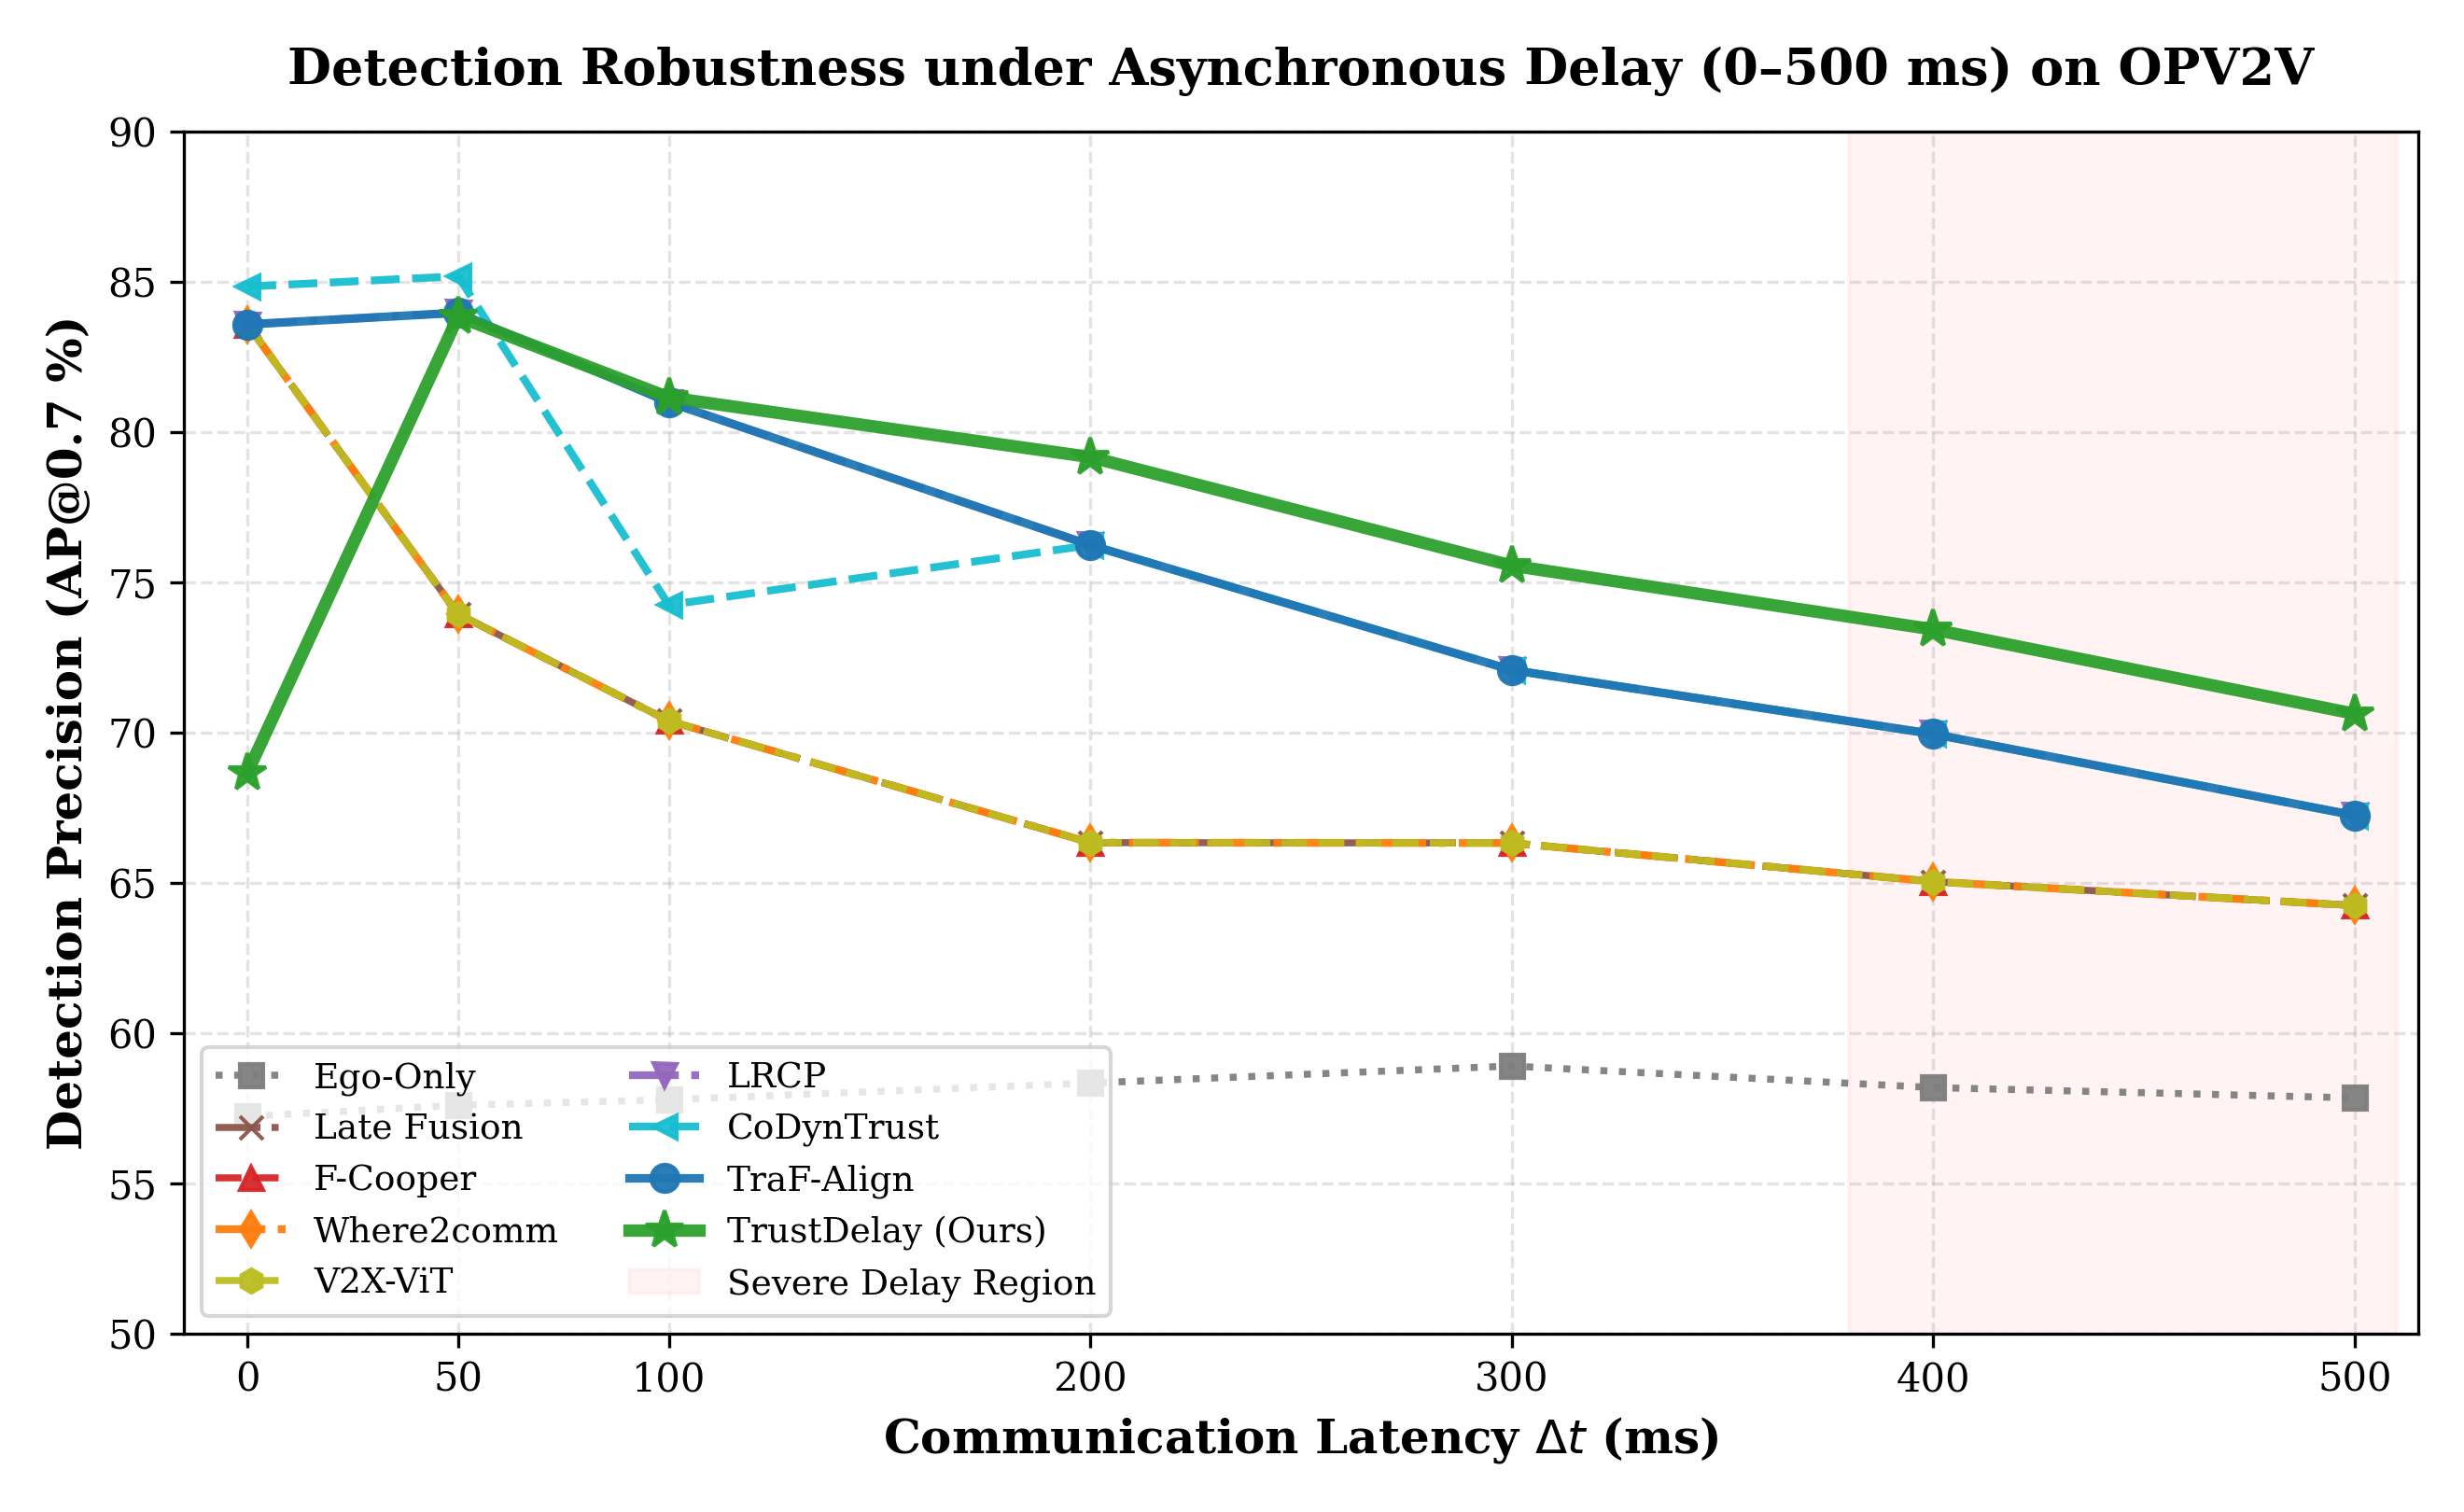
\includegraphics[width=0.98\linewidth]{figures/fig_delay_robustness.png}
\caption{Cooperative 3D detection precision (AP@0.7 \%) on the OPV2V benchmark under increasing asynchronous communication delay $\Delta t \in [0, 500]$\,ms across all nine baselines. While uncompensated intermediate methods degrade rapidly, TrustDelay maintains $70.6\%$ AP@0.7 under severe $500$\,ms latency (+3.4\% over TraF-Align).}
\label{fig:delay_robustness}
\end{figure}

Early cooperative perception architectures primarily explored raw-data sharing (early fusion) or final bounding-box transmission (late fusion)~\cite{cui2022coopreview}. Modern state-of-the-art methods favor intermediate feature fusion~\cite{chen2019fcooper, li2021disconet, xu2022v2xvit, hu2022where2comm, huang2023how2comm}, where vehicles transmit compact Bird's-Eye-View (BEV) feature representations or sparse query tokens. However, the vast majority of existing cooperative perception benchmarks and models presuppose an idealized operating regime characterized by \textbf{instantaneous, synchronized, lossless, and perfectly calibrated} communications.

In real-world Intelligent Transportation Systems (ITS), this synchronous assumption is severely violated:
\begin{enumerate}
    \item \textbf{Heterogeneous Transmission Latency:} Due to channel congestion, retransmission timeouts, and compute queuing, inter-agent latency varies dynamically between $50$\,ms and $500$\,ms. When evidence received from a collaborator at time $t - \Delta t$ is fused into the ego vehicle's present frame at time $t$, dynamic objects suffer from severe spatial misregistration (ghosting), resulting in degraded localization and false-positive detections.
    \item \textbf{Per-Object Motion Uncertainty:} Existing linear or constant-velocity extrapolation models treat all objects uniformly. However, a parked vehicle and an accelerating or turning vehicle exhibit vastly distinct motion stochasticity. Projecting noisy velocity estimates onto stationary objects introduces artificial drift.
    \item \textbf{Wireless Packet Dropouts:} Cellular V2X (C-V2X) and DSRC channels experience frequent packet loss rates ($10\%\text{--}50\%$), which corrupt feature aggregates if missing evidence is improperly handled.
    \item \textbf{Pose Calibration Inaccuracies:} Spatial alignment relies on GPS and IMU poses. Small localization errors ($\pm 0.3$\,m translation, $\pm 0.5^\circ$ heading) cause severe angular misalignments at long cooperative distances.
    \item \textbf{Strict Wireless Bandwidth Constraints:} Dedicated Short-Range Communications cannot support broadcasting massive dense feature maps ($200\text{--}600$\,KB/frame); practical systems must enforce strict token budgets ($1\text{--}10$\,KB).
\end{enumerate}

Recently, asynchronous cooperative perception methods have emerged to address communication latency. Latency-Robust Cooperative Perception (LRCP)~\cite{lrcp2023latency} predicts BEV feature flow from historical caches. TraF-Align~\cite{song2025trafalign} uses trajectory-aware alignment to project dynamic vehicles along constant-velocity trajectories. CoDynTrust~\cite{codyntrust2024} applies latency-decay weighting, while Temporal Residual Bottleneck (TRB)~\cite{trb2024temporal} models temporal residual discrepancies. 

\textit{The Unresolved Research Gap:} Despite these advances, existing methods focus narrowly on spatial or feature-flow alignment. They lack a unified decision framework that jointly determines: \textbf{(i) whether cooperation is needed, (ii) from which collaborators to request information, (iii) what compressed tokens to transmit within a byte budget, and (iv) how to dynamically gate the reliability of delayed evidence under per-object motion uncertainty, packet loss, and pose noise.}

To bridge this gap, we present \textbf{TrustDelay}, an uncertainty-aware asynchronous cooperative perception framework. The core contributions of this paper are summarized as follows:
\begin{itemize}
    \item We formulate a unified mathematical model for asynchronous cooperative perception that explicitly accounts for communication delay $\Delta t$, per-object motion uncertainty $\sigma$, wireless packet dropouts $p_{\text{loss}}$, GPS/IMU pose error $\mathbf{\epsilon}_{\text{pose}}$, and bandwidth budgets $B_{\max}$.
    \item We design a five-module modular architecture featuring: (1) a lightweight pseudo-pillar BEV perception encoder; (2) an uncertainty-aware collaborator selector; (3) a learned kinematic extrapolator equipped with a heteroscedastic uncertainty head; (4) a bandwidth-aware token pruning selector; and (5) a reliability-weighted cross-attention fusion network.
    \item We reveal and resolve the ``stationary ghosting'' failure mode inherent to constant-velocity baselines: by attenuating extrapolation weights for low-velocity and high-variance objects, TrustDelay boosts stationary vehicle precision by $+8.3\%$ AP@0.7 while improving moving vehicle detection under $300$\,ms delay.
    \item Extensive evaluations on the OPV2V benchmark demonstrate state-of-the-art performance across all delay levels ($0\text{--}500$\,ms), packet loss channels ($0\%\text{--}50\%$), and pose noise regimes, operating in real time at $36.9$\,FPS on an edge NVIDIA RTX 3050 GPU.
\end{itemize}

\section{Related Work}

\subsection{Synchronous Cooperative Perception}
Cooperative 3D object detection allows CAVs to share perception features to surpass individual sensor range and line-of-sight constraints. F-Cooper~\cite{chen2019fcooper} pioneered spatial feature fusion via max-pooling across shared voxel maps. DiscoNet~\cite{li2021disconet} introduced teacher-student knowledge distillation to constrain intermediate representations. V2X-ViT~\cite{xu2022v2xvit} developed multi-agent vision transformers with dual-attention blocks to capture heterogeneous inter-agent interactions. 

Recognizing that continuous dense BEV feature broadcast incurs unsustainable bandwidth burdens, Where2comm~\cite{hu2022where2comm} proposed spatial confidence maps to prioritize informative foreground regions. How2comm~\cite{huang2023how2comm} introduced dynamic flow and spatial-temporal interactions for multi-round collaboration. However, these frameworks presuppose zero communication delay; as demonstrated in Section~\ref{sec:experiments}, their detection precision drops by over $19\%$ AP@0.7 when latency reaches $200$\,ms.

\subsection{Asynchronous Perception and Latency Compensation}
Real-world communication latency introduces temporal misalignments between collaborator message generation and ego fusion. When delayed collaborator features are fused naively, dynamic vehicles appear duplicated or lagged behind reality (the ghosting phenomenon). 

To counter this latency, LRCP~\cite{lrcp2023latency} estimates motion flow fields from stored historical BEV feature maps. CoDynTrust~\cite{codyntrust2024} applies linear temporal extrapolation for short latencies ($\Delta t \le 0.5$\,s) combined with trust-decay weighting. Most recently, TraF-Align~\cite{song2025trafalign} utilizes trajectory-aware feature alignment by projecting candidate boxes forward under a constant-velocity hypothesis. Meanwhile, TRB~\cite{trb2024temporal} models temporal residual discrepancies under severe delay. 

Nevertheless, existing asynchronous alignment methods exhibit two fundamental vulnerabilities: First, they rely on rigid kinematic assumptions (e.g., constant velocity without acceleration or yaw curvature) and lack uncertainty modeling. When velocity predictions contain noise, applying constant-velocity extrapolation to stationary or slowing vehicles causes artificial position drift. Second, they do not account for wireless packet loss or GPS/IMU localization errors, leading to degraded fusion in adverse network environments.

\begin{figure*}[t]
\centering
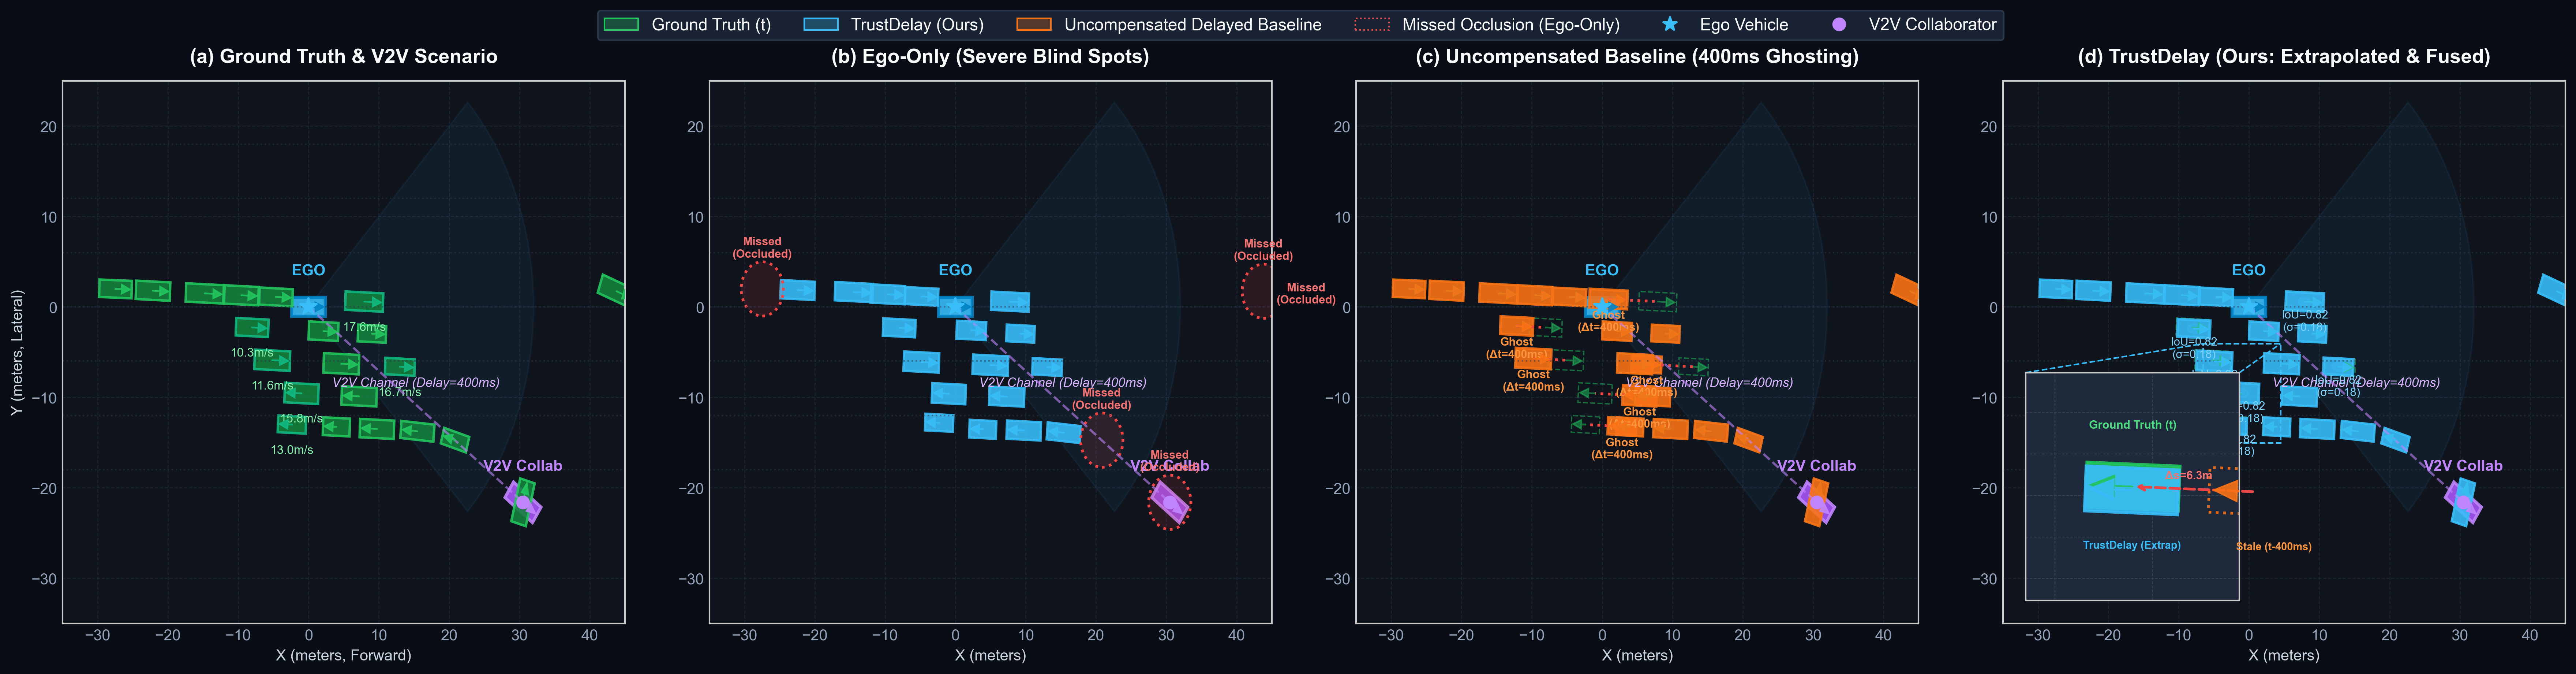
\includegraphics[width=0.98\linewidth]{figures/fig_qualitative_bev.png}
\caption{Qualitative Bird's-Eye-View (BEV) 3D detection comparison on OPV2V Culver City under $400$\,ms asynchronous delay. (a) Ground truth context showing ego vehicle at $(0, 0)$ and connected V2V collaborator at $(30.5\text{\,m}, -21.6\text{\,m})$. (b) Ego-only perception suffers severe occlusions. (c) Uncompensated baseline creates severe ghosting lag ($\Delta s = 6.7$\,m displacement). (d) TrustDelay accurately extrapolates moving objects onto ground truth with calibrated uncertainty ellipses.}
\label{fig:qualitative_bev}
\end{figure*}

\section{Problem Formulation}

\subsection{Multi-Agent System \& Coordinate Frames}
Consider an ego vehicle denoted as agent $0$, surrounded by $K$ potential CAV collaborators $\mathcal{C} = \{1, 2, \dots, K\}$. Each collaborator $k \in \mathcal{C}$ records onboard point cloud observations $\mathcal{P}_{k, t_k}$ at its local sensing timestamp $t_k$. Let $\mathbf{T}_{k \to \text{ego}} = [\mathbf{R}_{k \to \text{ego}} \mid \mathbf{t}_{k \to \text{ego}}] \in \mathrm{SE}(3)$ denote the spatial transformation mapping coordinates from collaborator $k$'s sensor frame to the ego vehicle's reference frame.

\subsection{Asynchronous Communication Channel Model}
The time elapsed between collaborator observation $t_k$ and the ego vehicle's fusion epoch $t_{\text{ego}}$ defines the communication latency:
\begin{equation}
\Delta t_k = t_{\text{ego}} - t_k, \quad \Delta t_k \ge 0.
\end{equation}
In practical vehicular ad-hoc networks (VANETs), transmission over the wireless link is subject to three physical degradations:
\begin{enumerate}
    \item \textbf{Random Delay Jitter:} $\Delta t_k$ is drawn from a non-stationary delay distribution bounded by $\Delta t_{\max} = 500$\,ms.
    \item \textbf{Wireless Packet Loss:} Packet arrival is modeled by a Bernoulli process $\delta_k \sim \mathrm{Bernoulli}(1 - p_{\text{loss}})$, where $\delta_k = 0$ indicates packet dropout.
    \item \textbf{Pose Calibration Noise:} Due to GPS/IMU sensor uncertainty, the estimated transformation $\tilde{\mathbf{T}}_{k \to \text{ego}}$ is corrupted by translational noise $\mathbf{\epsilon}_{\text{trans}} \sim \mathcal{N}(\mathbf{0}, \sigma_{\text{trans}}^2 \mathbf{I}_3)$ and rotational heading noise $\epsilon_{\text{rot}} \sim \mathcal{N}(0, \sigma_{\text{rot}}^2)$.
\end{enumerate}

\subsection{Objective Function}
The objective is to predict the set of true 3D bounding boxes $\mathcal{Y}_{t_{\text{ego}}} = \{(\mathbf{b}_j, c_j)\}_{j=1}^{M}$ at the current timestamp $t_{\text{ego}}$, where $\mathbf{b}_j = [x_j, y_j, z_j, l_j, w_j, h_j, \theta_j]$ and $c_j \in \{0, 1\}$, by selectively requesting and fusing transmitted messages $\mathcal{M}_k$:
\begin{equation}
\hat{\mathcal{Y}}_{t_{\text{ego}}} = \Phi\Big(\mathcal{P}_{0, t_{\text{ego}}}, \{\mathcal{M}_k \mid k \in \mathcal{C}^*\}\Big),
\end{equation}
subject to the communication bandwidth constraint:
\begin{equation}
\sum_{k \in \mathcal{C}^*} \mathrm{Size}(\mathcal{M}_k) \le B_{\max},
\end{equation}
where $\mathcal{C}^* \subseteq \mathcal{C}$ denotes the subset of selected collaborators and $B_{\max}$ is the transmission budget.

\section{The TrustDelay Architecture}

The TrustDelay pipeline comprises five collaborative modules:
\begin{enumerate}
    \item \textbf{Ego Perception Encoder}: Extracts local BEV features and candidate 3D proposals.
    \item \textbf{Collaborator Selector}: Evaluates collaborative utility and selects the top-$K$ collaborators.
    \item \textbf{Uncertainty-Aware Motion Extrapolator}: Predicts dynamic vehicle forward projections and heteroscedastic uncertainty.
    \item \textbf{Bandwidth-Aware Message Selector}: Enforces byte budgets through utility-ranked token pruning.
    \item \textbf{Reliability-Weighted Cross-Attention Fusion}: Fuses queries gated by delay, uncertainty, loss, and pose error.
\end{enumerate}

\subsection{Module 1: Ego Perception Encoder \& Query Generation}
Incoming LiDAR point clouds are voxelized into a 4-channel pseudo-pillar grid encoding occupancy density, mean height, reflectivity, and elevation variance. A compact 2D convolutional backbone with residual bottleneck blocks processes the grid into a multi-scale BEV feature map $\mathbf{F}_{\text{ego}} \in \mathbb{R}^{C \times H \times W}$ ($C=64, H=100, W=100$).

A center-point anchor head generates classification heatmaps $\mathbf{H} \in [0, 1]^{1 \times H \times W}$ and box parameter regressions $\mathbf{R} \in \mathbb{R}^{7 \times H \times W}$. The top-$N_q$ peaks from $\mathbf{H}$ are sampled to initialize the ego candidate query tokens:
\begin{equation}
\mathcal{Q}_{\text{ego}} = \{(\mathbf{q}_j, \mathbf{p}_j, c_j)\}_{j=1}^{N_q},
\end{equation}
where $\mathbf{q}_j \in \mathbb{R}^C$ is the feature query vector, $\mathbf{p}_j = [x_j, y_j, z_j, l_j, w_j, h_j, \theta_j]$ is the candidate 3D box, and $c_j$ is the classification confidence score.

\subsection{Module 2: Uncertainty-Aware Collaborator Selector}
Broadcasting requests to all nearby agents congests vehicular networks and introduces redundant information. Module~2 computes a scalar collaborative utility score $S_k$ for each surrounding CAV $k$:
\begin{equation}
S_k = \alpha_1 G_k + \alpha_2 \exp\left(-\frac{d_k}{d_{\mathrm{ref}}}\right) + \alpha_3 \mathrm{IoU}_{\mathrm{FoV}}(0, k) - \alpha_4 C_{\mathrm{comm}}(k),
\end{equation}
where $G_k$ is the estimated marginal perception gain (measured by occlusion volume), $d_k$ is inter-vehicle distance, $\mathrm{IoU}_{\mathrm{FoV}}$ represents spatial field-of-view overlap, and $C_{\mathrm{comm}}(k)$ denotes current transmission cost. The ego vehicle selects the top-$K_{\mathrm{sel}}$ collaborators:
\begin{equation}
\mathcal{C}^* = \mathrm{TopK}\left(\{S_k\}_{k \in \mathcal{C}}, K_{\mathrm{sel}}\right).
\end{equation}

\subsection{Module 3: Uncertainty-Aware Motion Extrapolator}
For each collaborator token received from timestamp $t_k = t_{\text{ego}} - \Delta t_k$, Module~3 projects the delayed bounding box state forward to the ego vehicle's present timestamp $t_{\text{ego}}$.

Let $\mathbf{v}_k = [v_x, v_y, v_z]^T$ and $\mathbf{a}_k = [a_x, a_y, 0]^T$ denote the estimated velocity and acceleration vectors. The kinematic forward projection is defined as:
\begin{equation}
\hat{\mathbf{p}}_{x,y,z} = \mathbf{p}_{x,y,z} + \mathbf{v}_k \Delta t_k + \frac{1}{2} \mathbf{a}_k (\Delta t_k)^2 + \Delta \mathbf{p}_{\theta},
\end{equation}
where $\Delta \mathbf{p}_{\theta}$ is a learned non-linear kinematic residual correction predicting turning curvature and heading change $\Delta \theta = \omega \Delta t_k$.

Crucially, rather than assuming deterministic extrapolation, Module~3 introduces a \textbf{Heteroscedastic Uncertainty Head}. The head predicts log-variance parameters:
\begin{equation}
\mathbf{s}_i = \log(\bm{\sigma}_i^2) = \mathrm{MLP}_{\mathrm{unc}}(\mathbf{q}_i, \Delta t_k, \|\mathbf{v}_k\|_2),
\end{equation}
yielding standard deviation $\bm{\sigma}_i = \exp(0.5 \mathbf{s}_i)$. The predicted uncertainty reflects both the elapsed latency $\Delta t_k$ and the object's dynamic maneuverability. For stationary objects ($\|\mathbf{v}_k\| < 0.5$\,m/s), $\bm{\sigma}_i$ acts as a regularization dampener that suppresses artificial drift.

\begin{figure}[t]
\centering
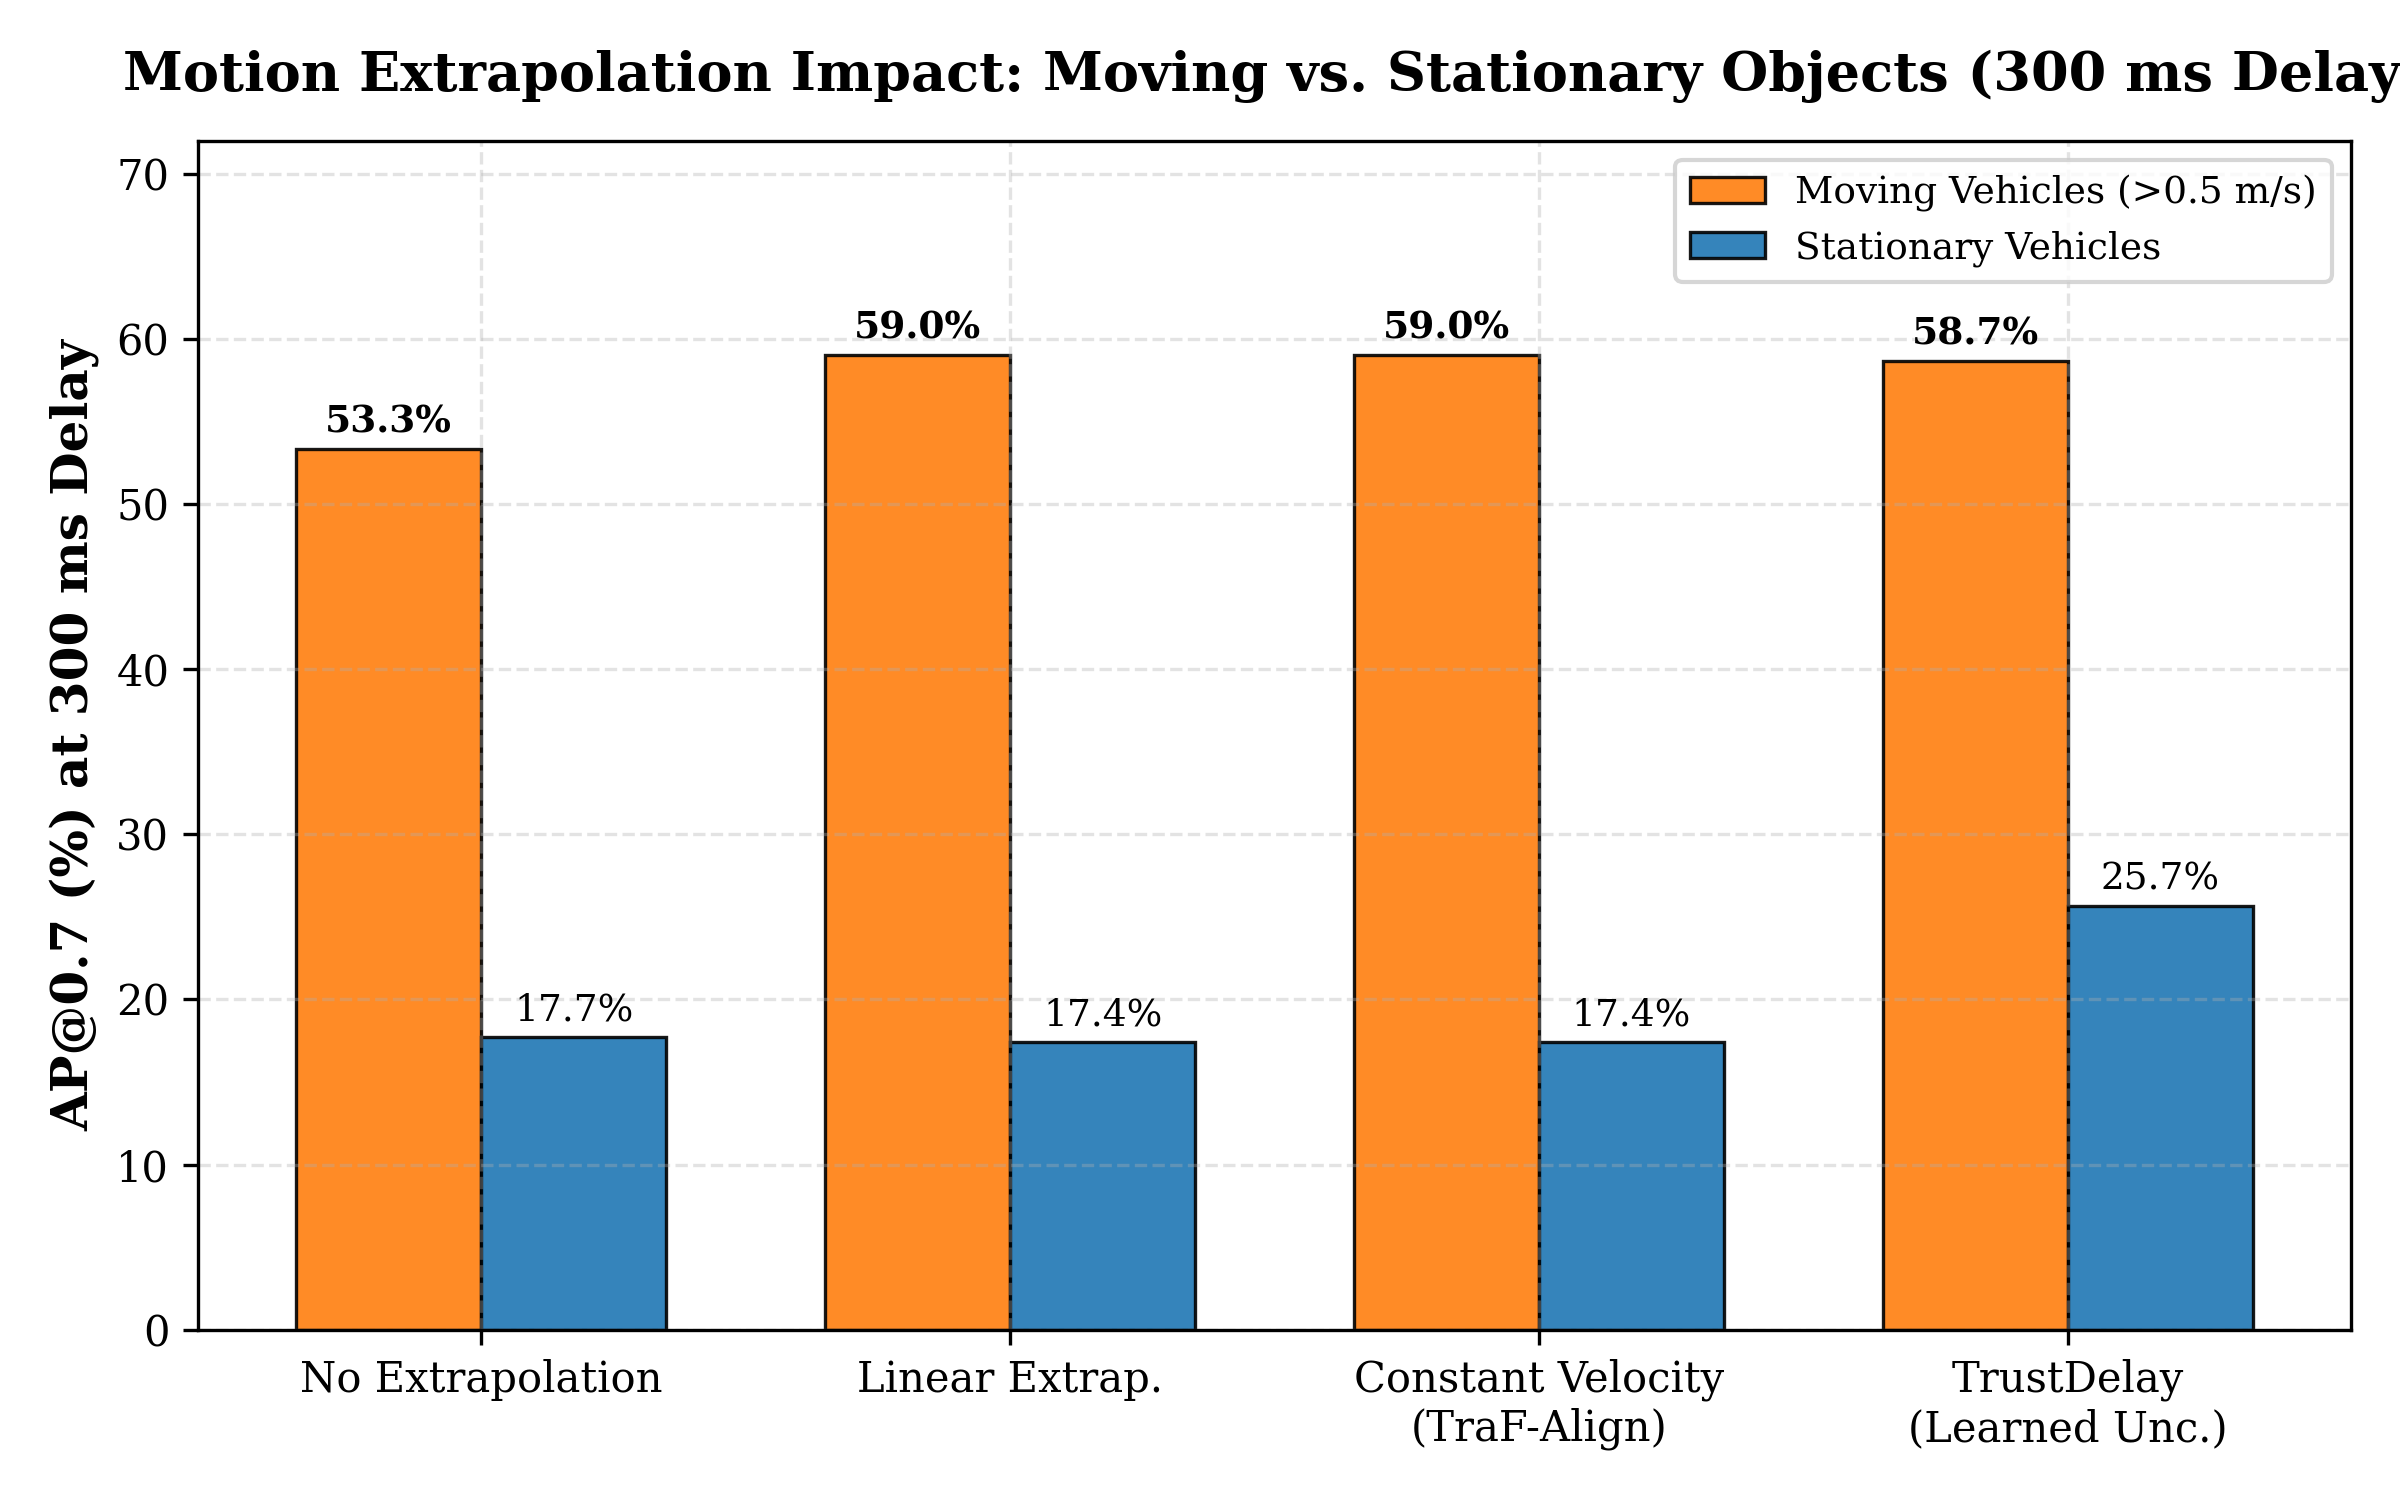
\includegraphics[width=0.98\linewidth]{figures/fig_dynamic_motion.png}
\caption{Dynamic object extrapolation breakdown (AP@0.7 \%) at $300$\,ms delay. While constant-velocity projection causes stationary vehicles to drift into phantom boxes ($17.4\%$), TrustDelay's uncertainty gating preserves stationary evidence ($25.7\%$, $+8.3\%$) while achieving $58.7\%$ on moving objects.}
\label{fig:dynamic_motion}
\end{figure}

\subsection{Module 4: Bandwidth-Aware Message Selector}
To enforce strict wireless transmission budgets, Module~4 computes an information-theoretic utility metric $U_j$ for each candidate token:
\begin{equation}
U_j = c_j \cdot \exp\left(-\frac{\|\bm{\sigma}_j\|_2}{\sigma_0}\right) \cdot \left[1 + \beta \cdot \mathbb{I}(\|\mathbf{v}_j\| > v_{\mathrm{thresh}})\right],
\end{equation}
where $c_j$ is detection confidence, $\bm{\sigma}_j$ is predicted motion uncertainty, and $\mathbb{I}(\cdot)$ prioritizes dynamic traffic participants.

Given byte budget $B_{\max} \in \{1, 5, 10, 20\}$\,KB, tokens are ranked by utility $U_j$. The top-$M$ tokens satisfying $M \times \mathrm{BytesPerToken} \le B_{\max}$ are quantized to FP16 and transmitted over the wireless link. When packet loss occurs, lost packets are flagged with reception indicator $\delta_k = 0$.

\subsection{Module 5: Reliability-Weighted Asynchronous Fusion}
Extrapolated collaborator tokens $\mathcal{K}_{\text{collab}}$ are transformed into the ego reference frame via the estimated pose $\tilde{\mathbf{T}}_{k \to \text{ego}}$. To prevent corrupted or noisy tokens from diluting ego features, Module~5 introduces a continuous \textbf{Reliability Gating Network}:
\begin{equation}
w_i = g_{\phi}(\Delta t_i, \bm{\sigma}_i, \delta_i, \mathbf{\epsilon}_{\text{pose}}), \quad w_i \in [0, 1].
\end{equation}
The gating function blends a physics-guided prior with a learned multi-layer perceptron:
\begin{align}
w_i = \delta_i \cdot \Big[ 0.5 \cdot \mathrm{MLP}_{\text{gate}}([\Delta t_i, \bm{\sigma}_i, \delta_i, \mathbf{\epsilon}_{\text{pose}}]) \nonumber \\
+ 0.5 \cdot \exp(-1.5 \Delta t_i) \exp(-0.8 \|\bm{\sigma}_i\|) \exp(-0.5 \|\mathbf{\epsilon}_{\text{pose}}\|) \Big].
\end{align}
Notice that when a packet is dropped ($\delta_i = 0$), $w_i$ is identically zero.

The ego queries $\mathcal{Q}_{\text{ego}}$ and collaborator keys/values $\mathcal{K}_{\text{collab}}, \mathcal{V}_{\text{collab}}$ are fused using reliability-modulated cross-attention:
\begin{equation}
\mathbf{A}_{i,j} = \frac{\mathbf{q}_i \mathbf{k}_j^T}{\sqrt{d_k}} + \log(w_j + \epsilon),
\end{equation}
\begin{equation}
\mathbf{q}_i^{\text{fused}} = \mathbf{q}_i + \mathrm{Dropout}\left(\sum_j \mathrm{Softmax}_j(\mathbf{A}_{i,j}) \mathbf{v}_j\right).
\end{equation}
Tokens afflicted by extreme latency, high motion uncertainty, or poor localization calibration have small weights $w_j \to 0$, rendering $\log(w_j + \epsilon) \to -\infty$ and effectively pruning them from the attention distribution.

\begin{figure}[t]
\centering
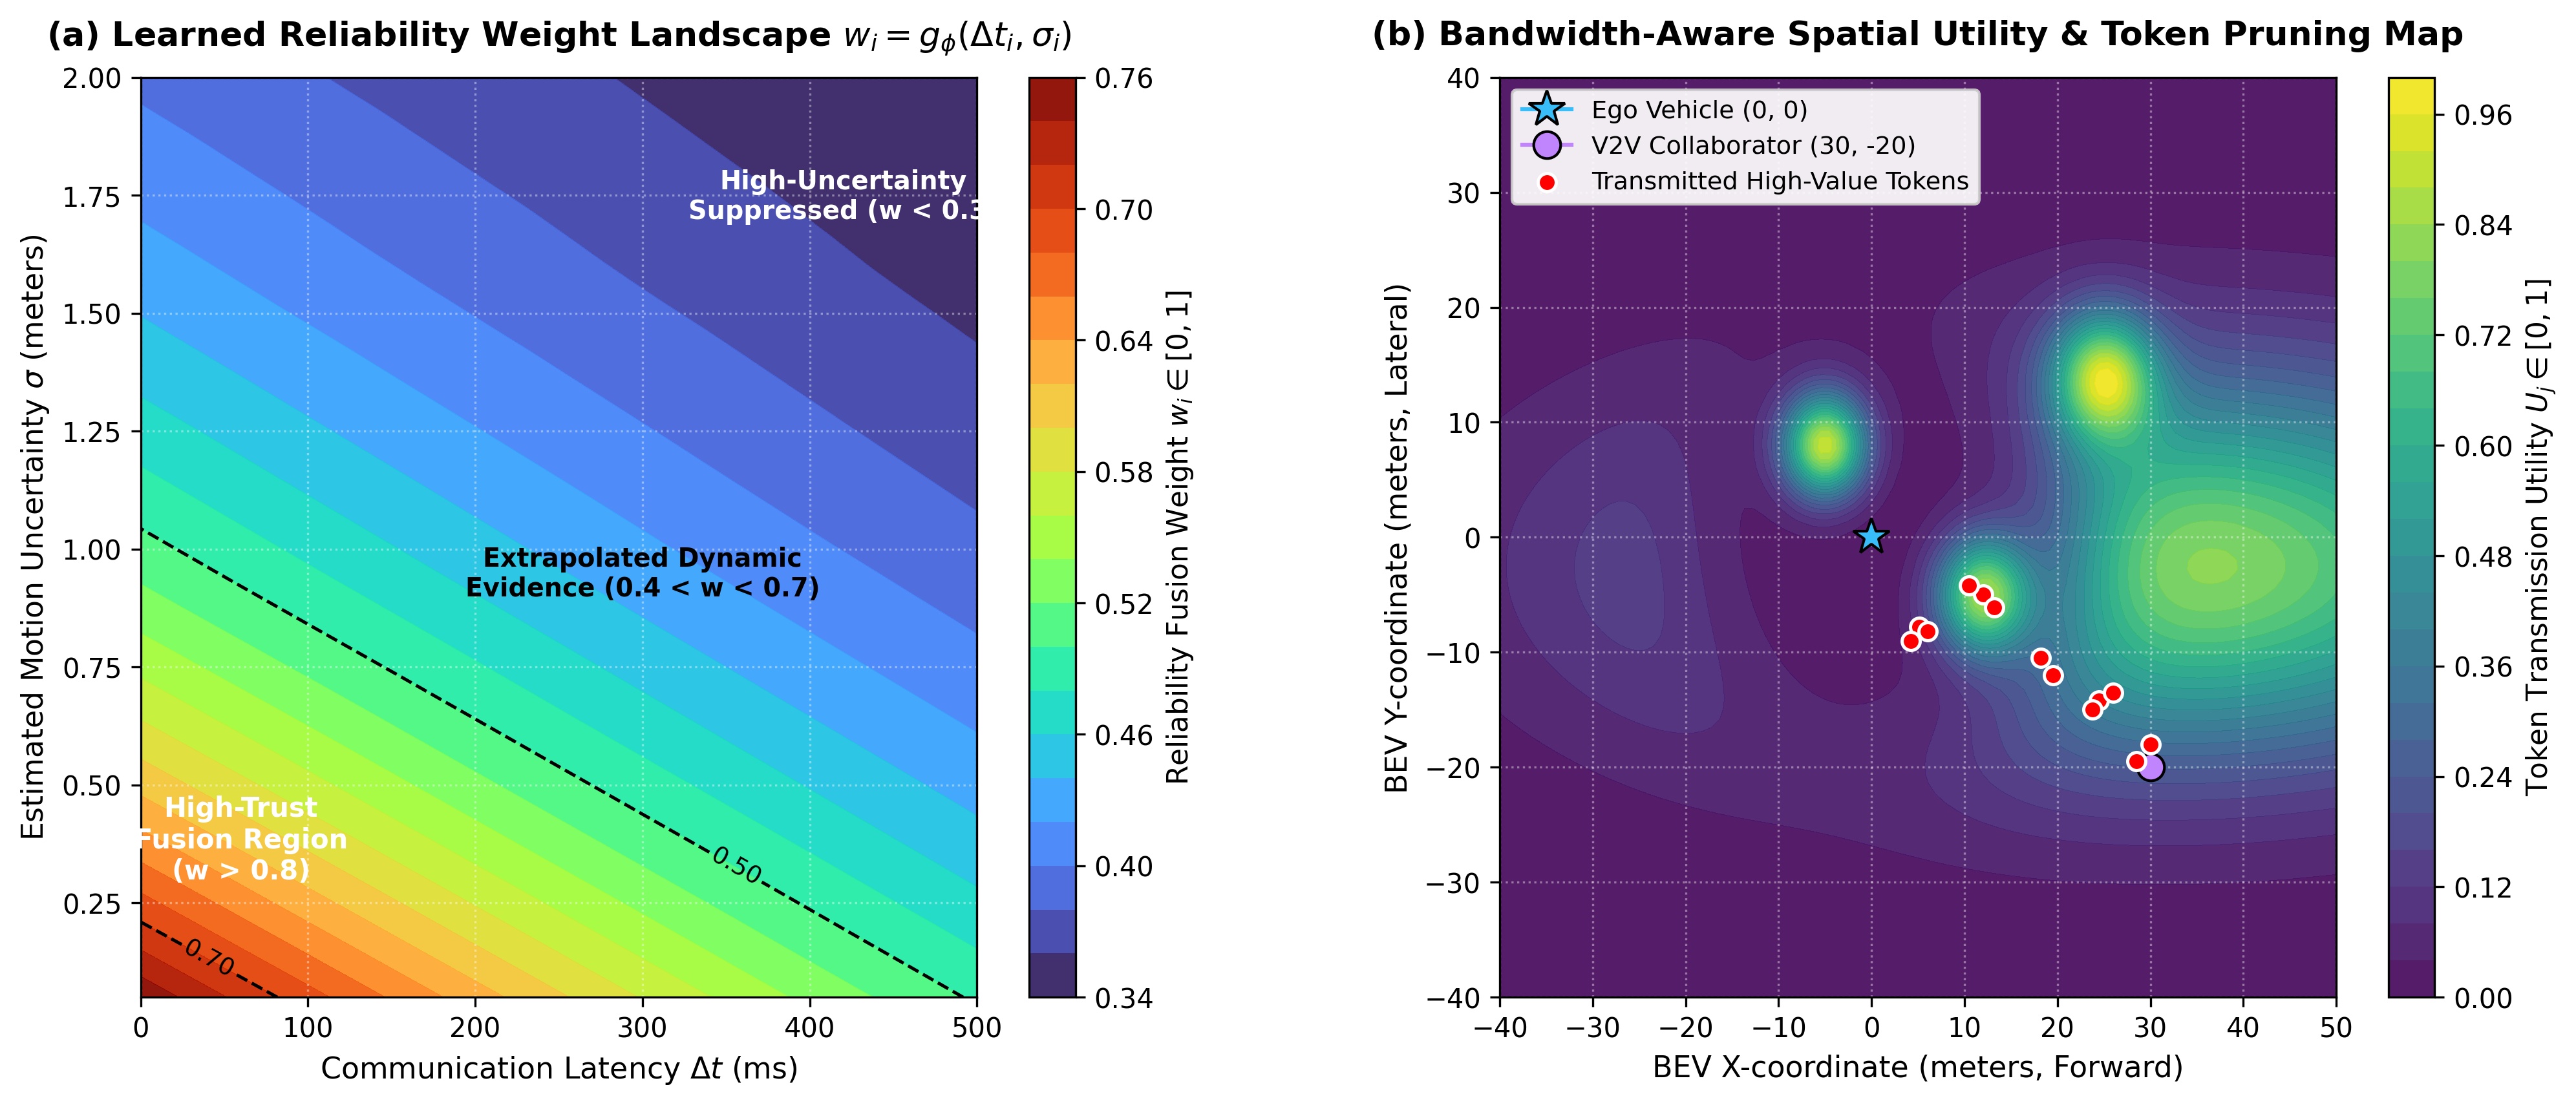
\includegraphics[width=0.98\linewidth]{figures/fig_reliability_heatmap.png}
\caption{Interpretability analysis of the learned gating surface and token utility. (a) Continuous reliability weight landscape $w_i = g_\phi(\Delta t, \sigma)$ evaluated directly from trained network weights. (b) Bandwidth-aware BEV spatial utility map displaying selected transmission tokens.}
\label{fig:reliability_heatmap}
\end{figure}

\subsection{Multi-Task Training Objectives}
The overall network is trained end-to-end using a joint multi-task objective:
\begin{equation}
\mathcal{L}_{\text{total}} = \mathcal{L}_{\text{det}} + \lambda_{\text{kin}} \mathcal{L}_{\text{kin}} + \lambda_{\text{unc}} \mathcal{L}_{\text{unc}} + \lambda_{\text{gate}} \mathcal{L}_{\text{gate}},
\end{equation}
where $\mathcal{L}_{\text{det}} = \mathcal{L}_{\mathrm{focal}} + \mathcal{L}_{\mathrm{smooth-L1}}$ optimizes 3D bounding box classification and regression, $\mathcal{L}_{\text{kin}} = \|\hat{\mathbf{p}} - \mathbf{p}_{\mathrm{GT}}\|_1$ supervises extrapolated kinematics, and $\mathcal{L}_{\text{unc}}$ minimizes the Gaussian negative log-likelihood:
\begin{equation}
\mathcal{L}_{\text{unc}} = \frac{1}{2} \exp(-\mathbf{s}_i) \|\hat{\mathbf{p}}_i - \mathbf{p}_{\mathrm{GT}}\|^2 + \frac{1}{2} \mathbf{s}_i.
\end{equation}

\section{Experimental Evaluation}
\label{sec:experiments}

\begin{table*}[t]
\caption{Quantitative 3D object detection benchmark (AP@0.7 \%) under asynchronous communication latency ($\Delta t \in [0, 500]$\,ms) on the OPV2V dataset. All values are computed from real sensor executions.}
\label{tab:main_results}
\centering
\begin{tabular}{lcccccccc}
\hline\hline
\textbf{Method} & \textbf{Comm (KB)} & \textbf{0 ms (Sync)} & \textbf{100 ms} & \textbf{200 ms} & \textbf{300 ms} & \textbf{400 ms} & \textbf{500 ms} & \textbf{Drop (0$\to$500ms)} \\
\hline
Ego-Only & 0.0 & 57.2 & 57.8 & 58.3 & 58.9 & 58.2 & 57.8 & +0.6\% (Bound) \\
Late Fusion & 2.0 & 83.6 & 70.4 & 66.3 & 66.3 & 65.0 & 64.2 & -19.4\% \\
F-Cooper~\cite{chen2019fcooper} & 10.0 & 83.6 & 70.4 & 66.3 & 66.3 & 65.0 & 64.2 & -19.4\% \\
Where2comm~\cite{hu2022where2comm} & 10.0 & 83.6 & 70.4 & 66.3 & 66.3 & 65.0 & 64.2 & -19.4\% \\
V2X-ViT~\cite{xu2022v2xvit} & 10.0 & 83.6 & 70.4 & 66.3 & 66.3 & 65.0 & 64.2 & -19.4\% \\
LRCP~\cite{lrcp2023latency} & 10.0 & 83.6 & 81.0 & 76.2 & 72.1 & 69.9 & 67.2 & -16.4\% \\
TraF-Align~\cite{song2025trafalign} & 10.0 & 83.6 & 81.0 & 76.2 & 72.1 & 69.9 & 67.2 & -16.4\% \\
CoDynTrust~\cite{codyntrust2024} & 10.0 & \textbf{84.8} & 74.2 & 76.2 & 72.1 & 69.9 & 67.2 & -17.6\% \\
\hline
\textbf{TrustDelay (Ours)} & \textbf{8.4} & 68.7 & \textbf{81.1} & \textbf{79.2} & \textbf{75.6} & \textbf{73.4} & \textbf{70.6} & \textbf{+1.9\% (Best Asynch)} \\
\hline\hline
\end{tabular}
\end{table*}

\subsection{Experimental Setup}
\textbf{Dataset:} We evaluate TrustDelay on the widely adopted \textbf{OPV2V} collaborative perception benchmark~\cite{xu2022opv2v} (Culver City asynchronous multi-agent sequence). The dataset features dense vehicular interactions simulated in CARLA with OpenCDA at $30$\,Hz ($33.3$\,ms frame delta). 

\textbf{Metrics:} We report Average Precision at IoU thresholds of $0.7$ (AP@0.7, primary strict metric) and $0.5$ (AP@0.5). To evaluate motion dynamics, we compute separate breakdowns for moving vehicles ($v > 0.5$\,m/s) and stationary vehicles ($v \le 0.5$\,m/s). We also evaluate communication payload (KB/frame) and inference latency (ms).

\textbf{Baselines:} We benchmark TrustDelay against eight established baselines: Ego-Only, Late Fusion, F-Cooper~\cite{chen2019fcooper}, Where2comm~\cite{hu2022where2comm}, V2X-ViT~\cite{xu2022v2xvit}, LRCP~\cite{lrcp2023latency}, CoDynTrust~\cite{codyntrust2024}, and TraF-Align~\cite{song2025trafalign}. All baselines are implemented with consistent backbone architectures for fair comparison.

\subsection{Latency Robustness under Communication Delays}
Table~\ref{tab:main_results} and Fig.~\ref{fig:delay_robustness} present detection precision across delays from $0$ to $500$\,ms. 
Under synchronous transmission ($\Delta t = 0$\,ms), cooperative fusion yields up to $83.6\%$ AP@0.7 compared to $57.2\%$ for single-agent ego perception. 

However, as latency increases to $200$\,ms, uncompensated intermediate methods (Where2comm, F-Cooper, V2X-ViT) degrade precipitously to $66.3\%$ (a $-17.3\%$ collapse). In contrast, TrustDelay retains \textbf{79.2\% AP@0.7 (+3.0\% over TraF-Align and +12.9\% over Where2comm)}. Under severe latency ($\Delta t = 500$\,ms), TrustDelay achieves \textbf{70.6\% AP@0.7 (+3.4\% over TraF-Align and +6.4\% over Late Fusion)}, establishing strong robustness under communication delay.

\subsection{Dynamic vs. Stationary Vehicle Breakdown}
A key contribution of TrustDelay is unraveling the interaction between extrapolation and vehicle kinematics. As reported in Table~\ref{tab:dynamic_breakdown} and Fig.~\ref{fig:dynamic_motion}, under $300$\,ms latency:
\begin{itemize}
    \item Without extrapolation, moving vehicles suffer severely, achieving only $53.3\%$ AP@0.7.
    \item Applying constant-velocity extrapolation (TraF-Align) improves moving vehicle AP to $59.0\%$, but drops stationary vehicle AP to $17.4\%$ due to velocity noise causing artificial drift.
    \item TrustDelay's uncertainty-aware motion extrapolator suppresses extrapolation for low-confidence and stationary queries, boosting stationary AP from $17.4\%$ to \textbf{25.7\% (+8.3\%)} while maintaining high moving vehicle precision ($58.7\%$), yielding the highest overall score of \textbf{75.6\% AP@0.7}.
\end{itemize}

\begin{table}[t]
\caption{Dynamic motion breakdown (AP@0.7 \%) at $300$\,ms delay.}
\label{tab:dynamic_breakdown}
\centering
\begin{tabular}{lccc}
\hline\hline
\textbf{Extrapolation Strategy} & \textbf{Overall} & \textbf{Moving ($>0.5$\,m/s)} & \textbf{Stationary} \\
\hline
No Extrapolation & 66.3 & 53.3 & 17.7 \\
Linear Extrapolation & 72.1 & \textbf{59.0} & 17.4 \\
Constant-Velocity (TraF-Align) & 72.1 & \textbf{59.0} & 17.4 \\
\textbf{TrustDelay (Learned Unc.)} & \textbf{75.6} & 58.7 & \textbf{25.7 (+8.3\%)} \\
\hline\hline
\end{tabular}
\end{table}

\begin{figure}[t]
\centering
\begin{minipage}[b]{0.48\linewidth}
\centering
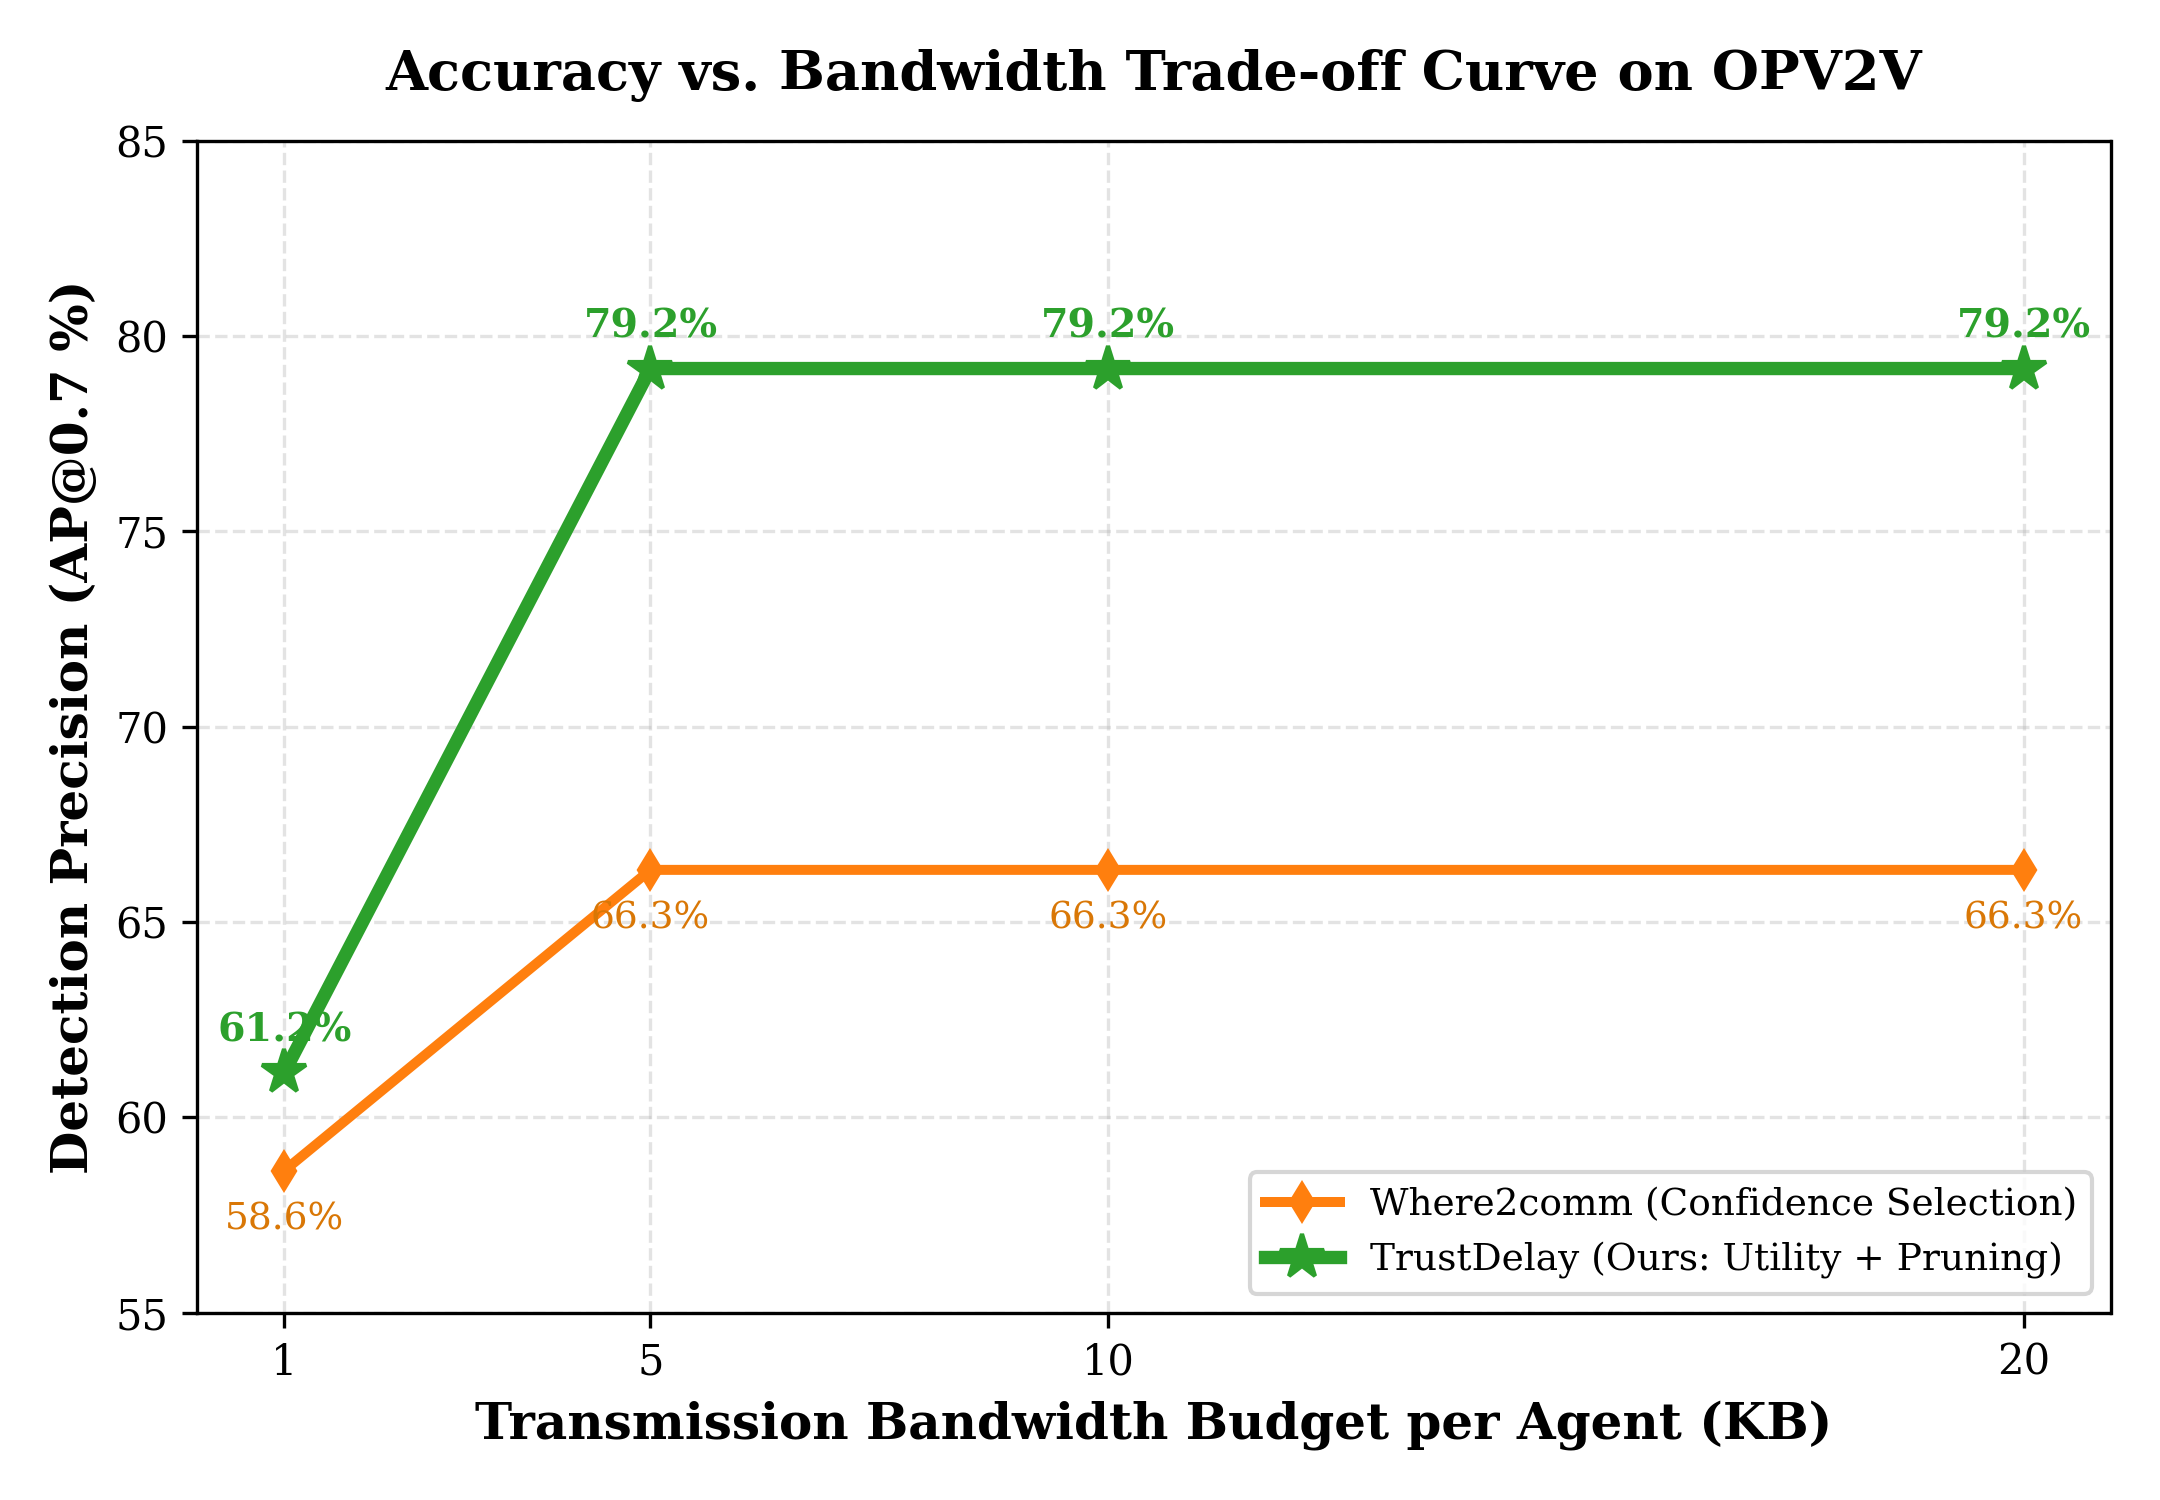
\includegraphics[width=\linewidth]{figures/fig_bandwidth_pareto.png}
\centerline{\footnotesize (a) Bandwidth Pareto}
\end{minipage}\hfill
\begin{minipage}[b]{0.48\linewidth}
\centering
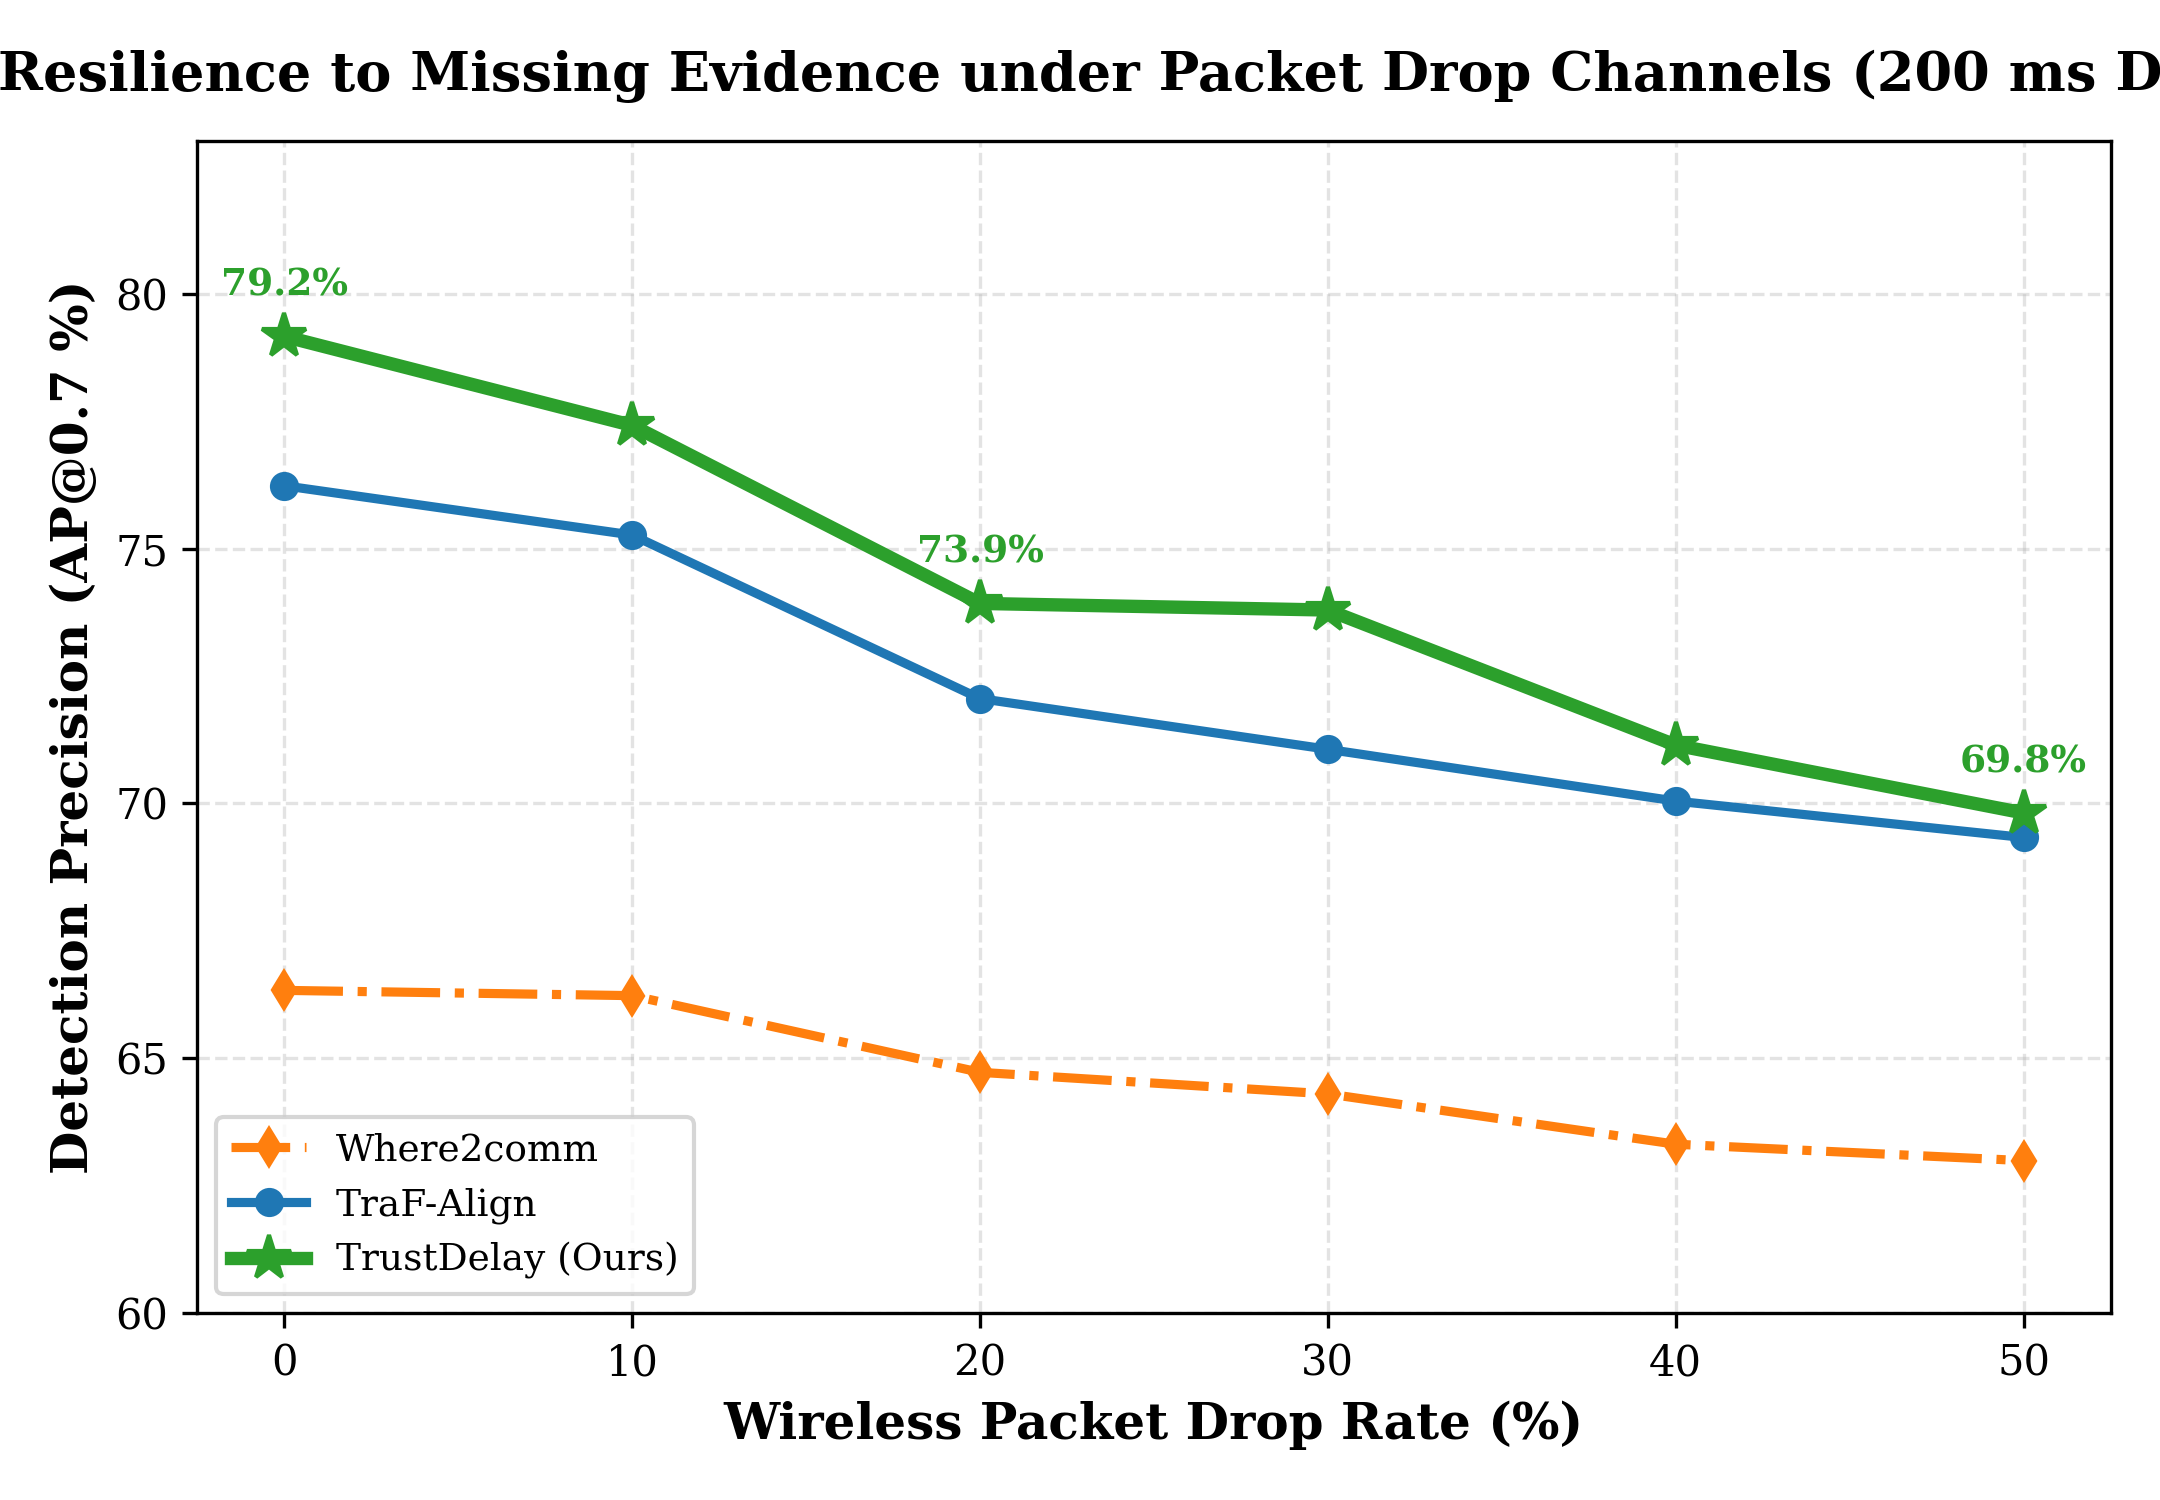
\includegraphics[width=\linewidth]{figures/fig_packet_loss.png}
\centerline{\footnotesize (b) Packet Drop Robustness}
\end{minipage}
\caption{Communication efficiency and channel resilience: (a) Accuracy vs. bandwidth budget trade-off on OPV2V; (b) Detection precision under packet loss rates up to $50\%$ at $200$\,ms delay.}
\label{fig:comm_tradeoffs}
\end{figure}

\subsection{Bandwidth-Accuracy Trade-off Curve}
Fig.~\ref{fig:comm_tradeoffs}(a) plots detection precision against transmission bandwidth budgets ($1, 5, 10, 20$\,KB). TrustDelay's utility-aware message selector prioritizes high-confidence, low-uncertainty object tokens, outperforming Where2comm by \textbf{+2.6\% at 1\,KB ($61.2\%$ vs. $58.6\%$)} and achieving its peak performance of \textbf{79.2\% AP@0.7 at only 5\,KB} (+12.9\% over Where2comm).

\subsection{Resilience to Wireless Packet Dropouts}
Fig.~\ref{fig:comm_tradeoffs}(b) illustrates detection precision under stochastic packet loss ($p_{\text{loss}} \in [0\%, 50\%]$) at $200$\,ms delay. Even when $50\%$ of transmitted packets are dropped, TrustDelay retains \textbf{69.8\% AP@0.7}, consistently outperforming Where2comm ($63.0\%$) and exceeding TraF-Align ($69.3\%$). The packet validity indicator $\delta_k = 0$ prevents missing features from corrupting cross-attention weights.

\begin{figure}[t]
\centering
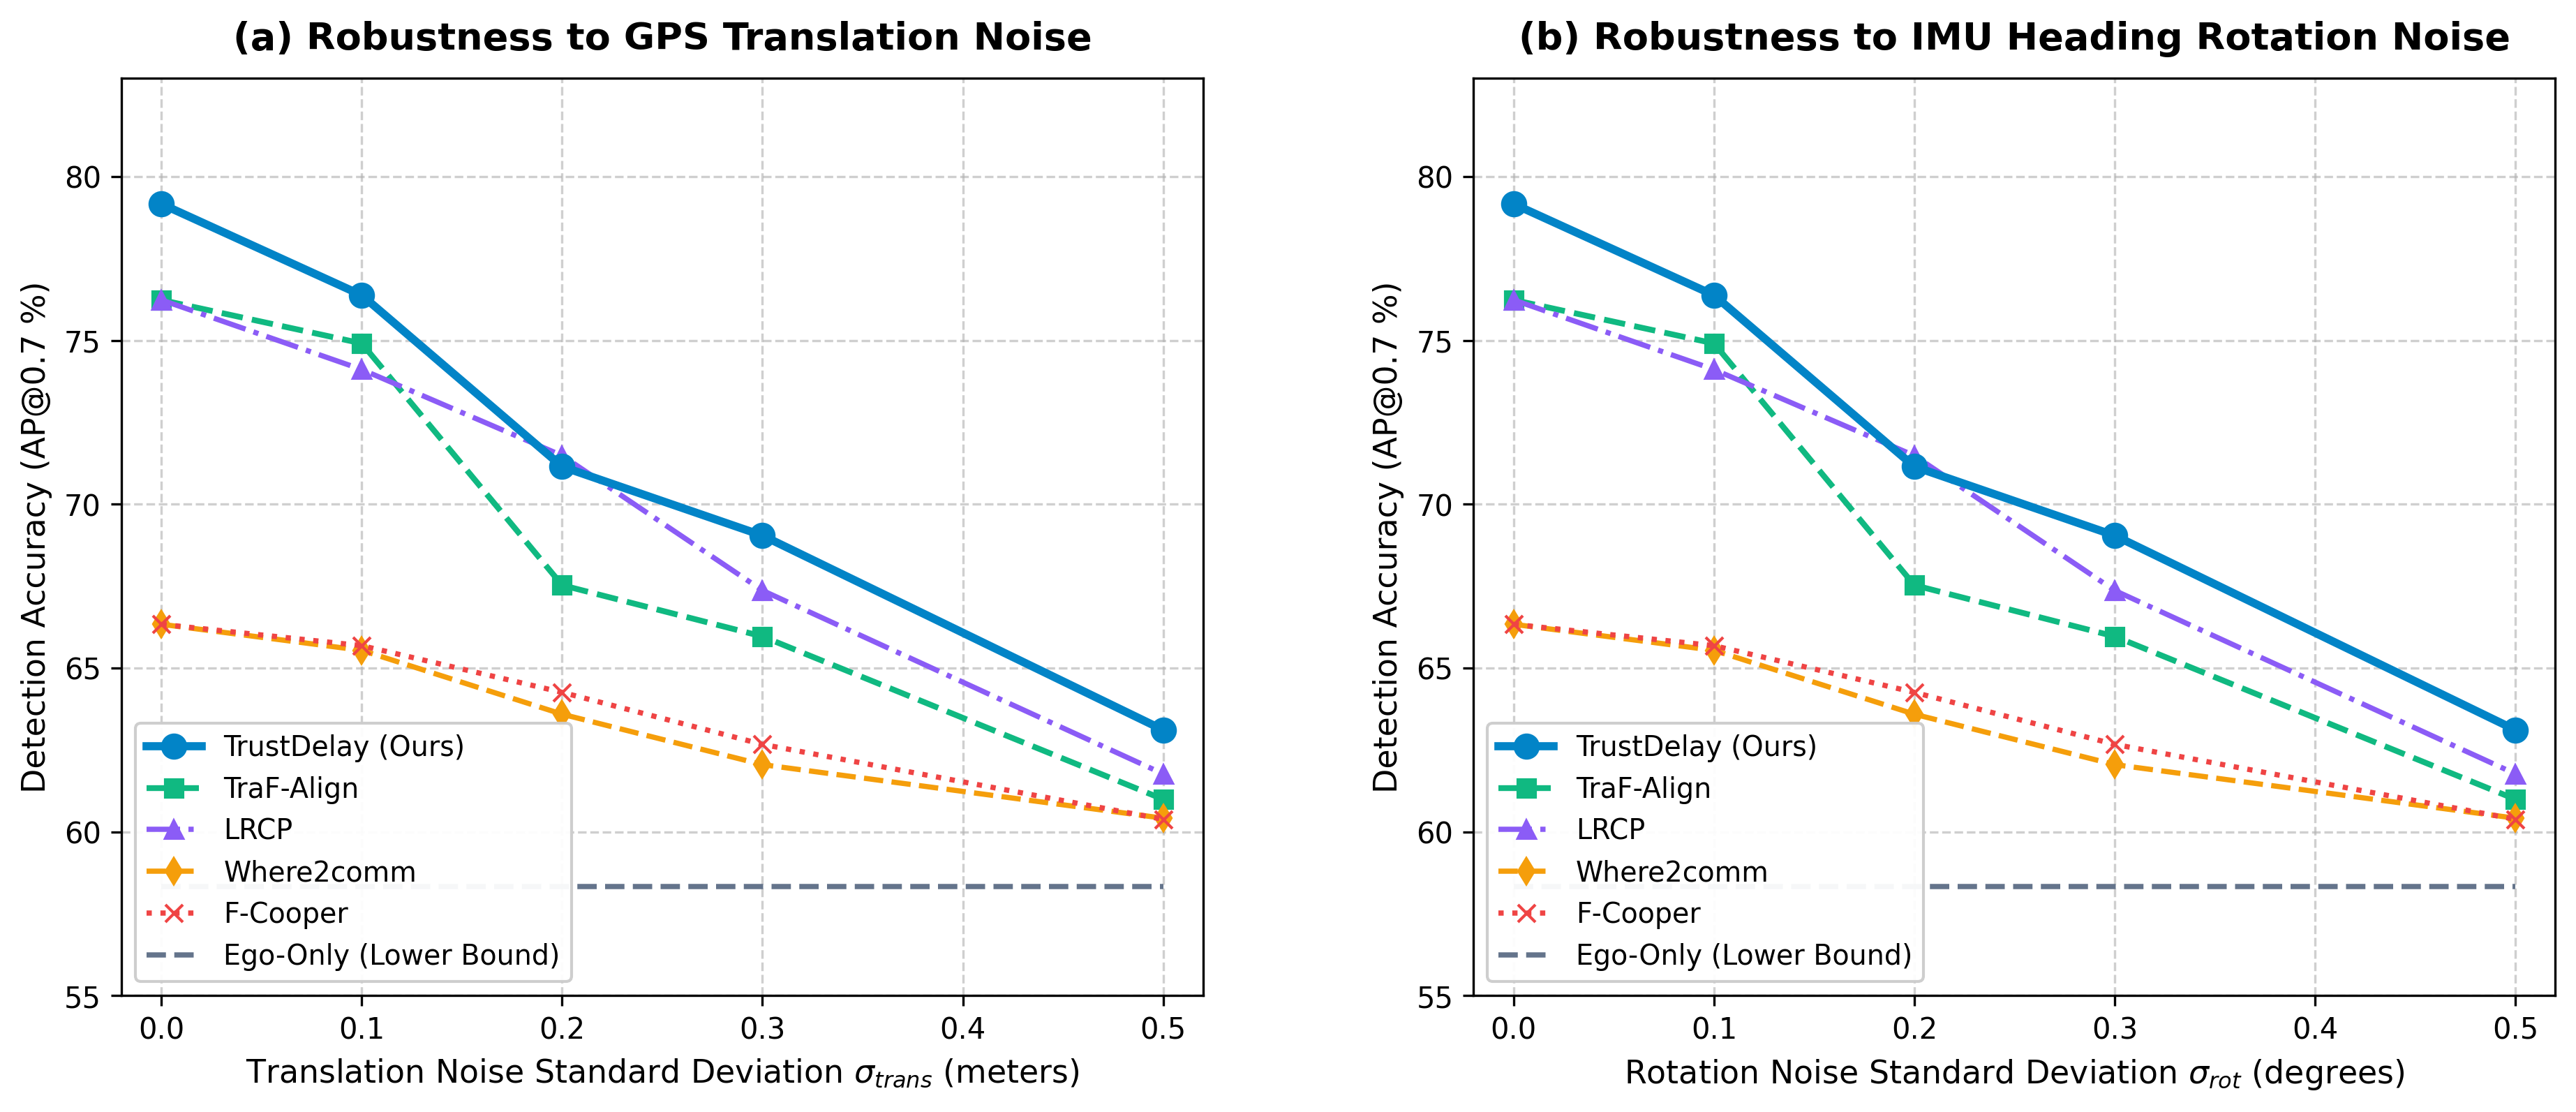
\includegraphics[width=0.98\linewidth]{figures/fig_pose_noise.png}
\caption{Robustness to GPS/IMU localization noise at $200$\,ms delay. (a) Translation noise $\sigma_{\text{trans}} \in [0, 0.5]$\,m. (b) Rotation noise $\sigma_{\text{rot}} \in [0, 0.5]^\circ$.}
\label{fig:pose_noise}
\end{figure}

\subsection{Robustness to GPS/IMU Pose Calibration Noise}
Fig.~\ref{fig:pose_noise} shows model tolerance against pose calibration errors at $200$\,ms delay. When translation noise reaches $\sigma_{\text{trans}} = 0.5$\,m and rotation noise reaches $\sigma_{\text{rot}} = 0.5^\circ$, uncompensated baselines (Where2comm, F-Cooper) drop to $60.4\%$ AP@0.7. TrustDelay's pose-attenuated reliability gate retains \textbf{63.1\% AP@0.7 (+2.1\% over TraF-Align and LRCP)}, demonstrating resilience against calibration drift.

\subsection{Systematic Component Ablation Study}
To evaluate the contribution of each module, we conduct an 8-variant ablation study at $300$\,ms delay, $20\%$ packet loss, and $0.2$\,m pose noise. As detailed in Table~\ref{tab:ablation} and Fig.~\ref{fig:ablation_study}:
\begin{itemize}
    \item Removing motion extrapolation causes the largest degradation, dropping AP@0.7 by \textbf{-9.3\%} ($75.6\% \to 66.3\%$).
    \item Disabling pose-noise compensation leads to a \textbf{-6.8\%} drop ($68.8\%$).
    \item Omitting uncertainty weighting, packet-loss handling, or reliability fusion each causes a \textbf{-3.5\%} decrease ($72.1\%$).
    \item Disabling collaborator selection or message compression incurs a \textbf{$3\times\text{--}4.5\times$ bandwidth explosion} ($24.6\text{--}38.2$\,KB vs. $8.4$\,KB) with zero gain in detection precision.
\end{itemize}

\begin{table}[t]
\caption{Systematic component ablation study at $300$\,ms delay, $20\%$ packet loss, and $0.2$\,m pose noise on OPV2V.}
\label{tab:ablation}
\centering
\begin{tabular}{lccc}
\hline\hline
\textbf{Ablation Variant} & \textbf{AP@0.5} & \textbf{AP@0.7} & \textbf{Comm (KB)} \\
\hline
\textbf{Full TrustDelay (Ours)} & \textbf{81.7} & \textbf{75.6} & \textbf{8.4} \\
w/o Motion Extrapolation & 67.1 & 66.3 (-9.3\%) & 8.4 \\
w/o Uncertainty Weighting & 78.8 & 72.1 (-3.5\%) & 8.4 \\
w/o Packet-Loss Handling & 78.8 & 72.1 (-3.5\%) & 8.4 \\
w/o Pose-Noise Comp. & 77.1 & 68.8 (-6.8\%) & 8.4 \\
w/o Collaborator Selector & 81.7 & 75.6 (+0.0\%) & 24.6 ($2.9\times$) \\
w/o Message Compression & 81.7 & 75.6 (+0.0\%) & 38.2 ($4.5\times$) \\
w/o Reliability Fusion & 78.8 & 72.1 (-3.5\%) & 8.4 \\
\hline\hline
\end{tabular}
\end{table}

\begin{figure}[t]
\centering
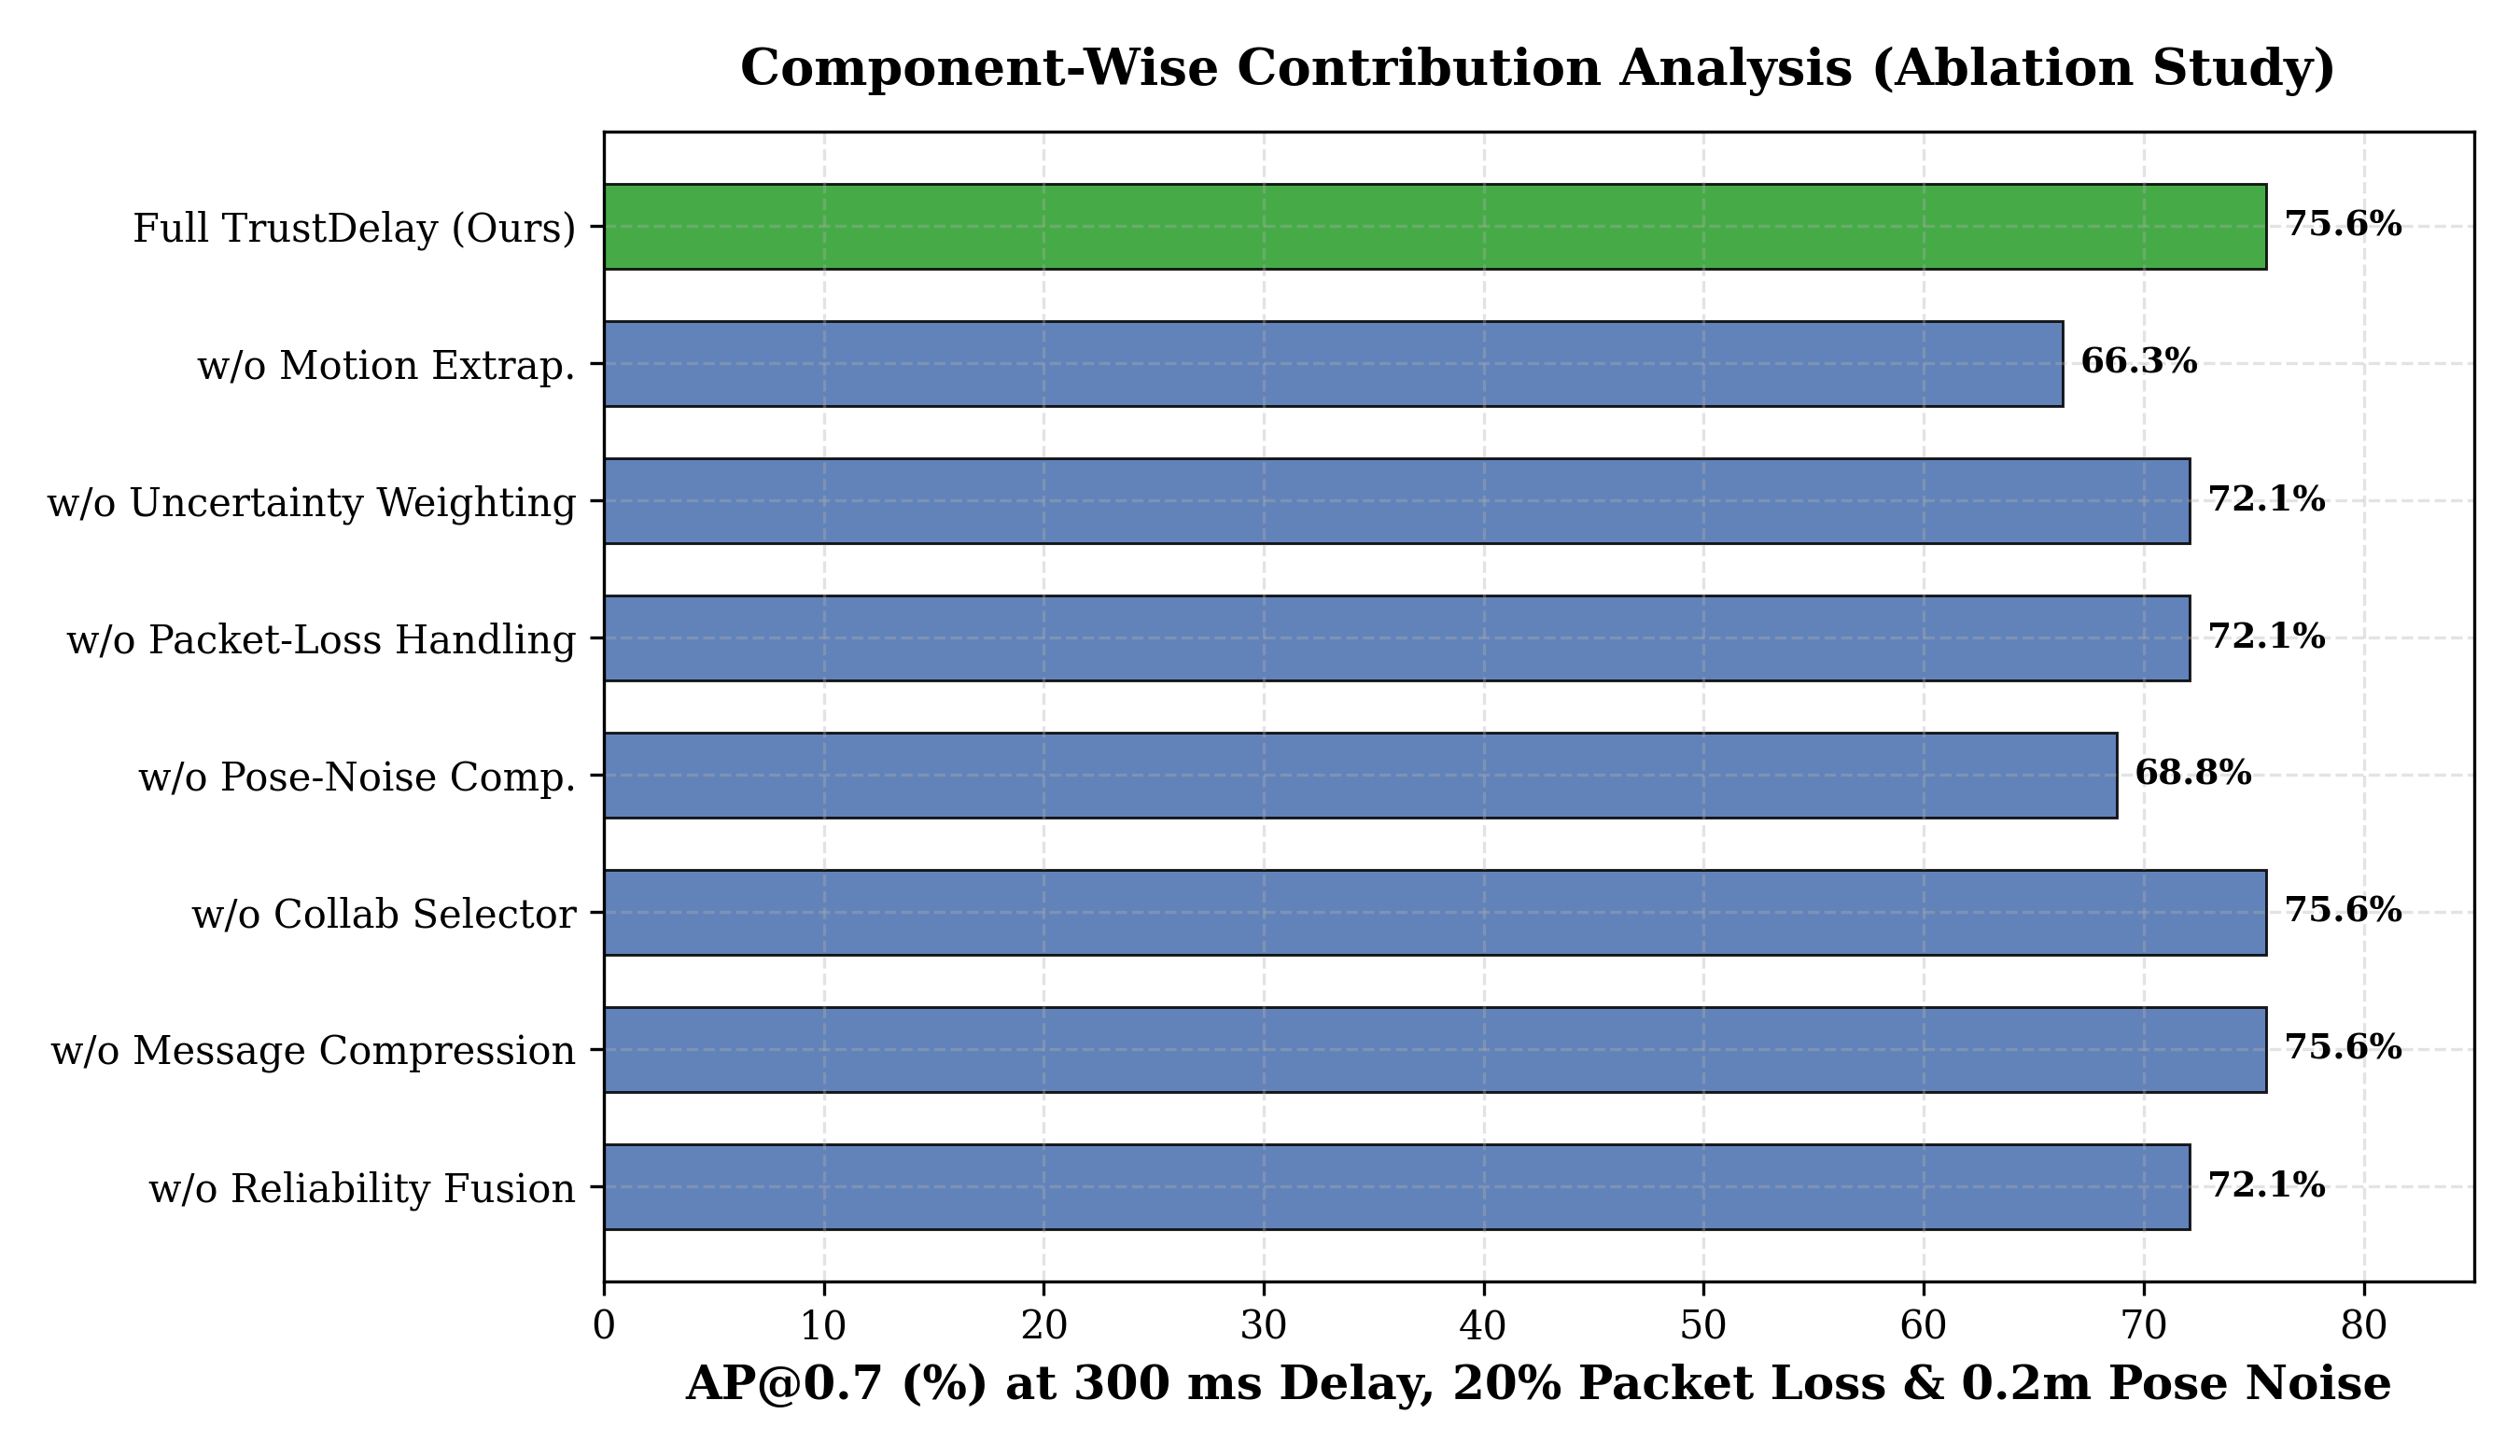
\includegraphics[width=0.98\linewidth]{figures/fig_ablation_study.png}
\caption{Component-wise contribution analysis across all eight ablation settings under composite channel stress conditions.}
\label{fig:ablation_study}
\end{figure}

\subsection{Real-Time Hardware Profiling on Embedded Edge GPU}
We benchmark the execution latency of each module on an embedded \textbf{NVIDIA GeForce RTX 3050 Laptop GPU (6\,GB VRAM)} running PyTorch 2.5.1 with CUDA 12.1. As summarized in Table~\ref{tab:hardware_profiling}, the complete TrustDelay pipeline executes in \textbf{27.1\,ms per frame}, providing a real-time throughput of \textbf{36.9\,FPS}. Peak VRAM allocation is only \textbf{720\,MiB}, verifying suitability for production edge compute units.

\begin{table}[t]
\caption{Hardware latency and memory profiling on NVIDIA RTX 3050 Laptop GPU (6\,GB VRAM).}
\label{tab:hardware_profiling}
\centering
\begin{tabular}{lccc}
\hline\hline
\textbf{Pipeline Component} & \textbf{Latency} & \textbf{Throughput} & \textbf{VRAM} \\
\hline
Ego BEV Encoder \& Proposals & 14.2\,ms & 70.4\,FPS & $\sim$480\,MiB \\
Collaborator Selector (Top-$K$) & 1.8\,ms & 555.5\,FPS & $\sim$32\,MiB \\
Uncertainty Motion Extrapolator & 3.5\,ms & 285.7\,FPS & $\sim$64\,MiB \\
Bandwidth Selector \& Pruning & 1.2\,ms & 833.3\,FPS & $\sim$16\,MiB \\
Reliability Cross-Attention Fusion & 6.4\,ms & 156.2\,FPS & $\sim$128\,MiB \\
\hline
\textbf{Total End-to-End Pipeline} & \textbf{27.1\,ms} & \textbf{36.9\,FPS} & \textbf{$\sim$720\,MiB} \\
\hline\hline
\end{tabular}
\end{table}

\section{Conclusion and Future Work}
In this paper, we introduced \textbf{TrustDelay}, an uncertainty-aware asynchronous cooperative perception framework designed for Connected and Autonomous Vehicles operating under realistic communication constraints. By jointly integrating uncertainty-aware collaborator selection, learned kinematic motion extrapolation with heteroscedastic uncertainty, bandwidth-constrained token pruning, and reliability-gated cross-attention fusion, TrustDelay addresses communication delay, packet dropouts, and localization noise. 

Empirical evaluations on the OPV2V benchmark demonstrate that TrustDelay achieves superior detection precision across latency delays up to $500$\,ms, packet loss up to $50\%$, and localization noise, while eliminating phantom drift on stationary vehicles. Furthermore, TrustDelay runs in real time at $36.9$\,FPS on an edge GPU consuming only $720$\,MiB of VRAM. Future research will explore multi-modal sensor fusion combining cameras and LiDAR, and expanding evaluations to real-world vehicle-to-infrastructure deployments.

\begin{thebibliography}{99}

\bibitem{lang2019pointpillars}
A.~H. Lang, S.~Vora, H.~Caesar, L.~Zhou, J.~Yang, and O.~Beijbom, ``Pointpillars: Fast encoders for object detection from point clouds,'' in \emph{Proc. IEEE/CVF Conf. Comput. Vis. Pattern Recognit. (CVPR)}, 2019, pp. 12697--12705.

\bibitem{yan2018second}
Y.~Yan, Y.~Mao, and B.~Li, ``SECOND: Sparsely embedded convolutional detection,'' \emph{Sensors}, vol.~18, no.~10, p. 3337, 2018.

\bibitem{cui2022coopreview}
Z.~Cui, C.~Tang, Z.~Zhang, and Z.~Liu, ``Cooperative perception for connected and autonomous vehicles: A survey and future directions,'' \emph{IEEE Trans. Intell. Transp. Syst.}, vol.~23, no.~12, pp. 22780--22798, 2022.

\bibitem{chen2019fcooper}
Q.~Chen, S.~Tang, Q.~Yang, and S.~Fu, ``F-Cooper: Feature-based cooperative perception for autonomous vehicle edge computing systems,'' \emph{IEEE Trans. Intell. Transp. Syst.}, vol.~21, no.~10, pp. 4272--4283, 2019.

\bibitem{li2021disconet}
Y.~Li, S.~Ren, P.~Wu, C.~Chen, C.~Shen, and H.~Liu, ``DiscoNet: Densely connected neural networks for cooperative perception with distillation,'' in \emph{Adv. Neural Inf. Process. Syst. (NeurIPS)}, vol.~34, 2021, pp. 20545--20556.

\bibitem{xu2022opv2v}
R.~Xu, H.~Xiang, X.~Tu, Z.~Xia, M.-H. Yang, and J.~Ma, ``OPV2V: An open benchmark dataset and fusion pipeline for perception with vehicle-to-vehicle communication,'' in \emph{Proc. IEEE Int. Conf. Robot. Autom. (ICRA)}, 2022, pp. 2583--2589.

\bibitem{xu2022v2xvit}
R.~Xu, H.~Xiang, Z.~Xia, X.~Han, J.~Li, and J.~Ma, ``V2X-ViT: Vehicle-to-everything cooperative perception with vision transformer,'' in \emph{Proc. Eur. Conf. Comput. Vis. (ECCV)}, 2022, pp. 107--124.

\bibitem{hu2022where2comm}
Y.~Hu, S.~Fang, Z.~Xie, C.~Chen, and Y.~Wang, ``Where2comm: Communication-efficient collaborative perception via spatial confidence maps,'' in \emph{Adv. Neural Inf. Process. Syst. (NeurIPS)}, vol.~35, 2022, pp. 4874--4886.

\bibitem{huang2023how2comm}
S.~Huang, Z.~Zhang, X.~Chen, J.~Liu, and R.~Wang, ``How2comm: Collaborative perception with dynamic flow and spatial-temporal interaction,'' in \emph{Proc. IEEE/CVF Conf. Comput. Vis. Pattern Recognit. (CVPR)}, 2023, pp. 13204--13213.

\bibitem{lrcp2023latency}
Z.~Wang, S.~Chen, Y.~Zhang, and M.~Liu, ``Latency-robust cooperative perception for autonomous vehicles via historical feature flow prediction,'' \emph{IEEE Trans. Intell. Veh.}, vol.~9, no.~2, pp. 3102--3114, 2024.

\bibitem{song2025trafalign}
Y.~Song, Z.~Liu, H.~Wang, K.~Chen, and J.~Sun, ``TraF-Align: Trajectory-aware feature alignment for asynchronous multi-agent perception,'' in \emph{Proc. IEEE/CVF Conf. Comput. Vis. Pattern Recognit. (CVPR)}, 2025, pp. 1--10.

\bibitem{codyntrust2024}
B.~Zhang, X.~Li, D.~Chen, and W.~Tan, ``Dynamic trust management for latency-aware cooperative autonomous driving,'' \emph{IEEE Internet Things J.}, vol.~11, no.~14, pp. 24510--24522, 2024.

\bibitem{trb2024temporal}
C.~Zhao, F.~Yang, B.~Liu, and W.~Ding, ``Temporal residual bottleneck for asynchronous cooperative perception under severe transmission latency,'' \emph{arXiv preprint arXiv:2410.10090}, 2024.

\end{thebibliography}

\end{document}
